\documentclass[12pt,a4paper]{report}
\usepackage{fontspec}
\setmainfont{Times New Roman}
\usepackage[top=2.5cm,bottom=2.5cm,left=3cm,right=2cm]{geometry}
\usepackage{amsmath,amssymb,booktabs,tabularx,array,multirow}
\usepackage{graphicx,float,xcolor,tikz}
\usetikzlibrary{calc,positioning,arrows.meta,shapes.geometric}
\usepackage{hyperref,xurl,fancyhdr,titlesec,caption,enumitem,longtable}
\usepackage{microtype}
\renewcommand{\contentsname}{Mục lục}
\renewcommand{\listfigurename}{Danh mục hình ảnh}
\renewcommand{\listtablename}{Danh mục bảng}
\renewcommand{\chaptername}{Chương}
\renewcommand{\figurename}{Hình}
\renewcommand{\tablename}{Bảng}
\renewcommand{\bibname}{Tài liệu tham khảo}
\makeatletter
\setlength{\@fptop}{0pt}
\setlength{\@fpsep}{12pt}
\setlength{\@fpbot}{0pt plus 1fil}
\makeatother
\hypersetup{colorlinks=true,linkcolor=blue!70!black,urlcolor=blue!70!black,citecolor=blue!70!black,pdftitle={Tieu luan 03 - Phan tich he thong thong minh: ML CNN RNN KG RAG},pdfauthor={Phan Van Khoi}}
\setlength{\parindent}{1.2cm}
\setlength{\parskip}{3pt}
\linespread{1.14}
\titleformat{\chapter}[display]{\normalfont\bfseries\color{blue!75!black}}{\filleft\Large\chaptertitlename\ \thechapter}{1ex}{\titlerule\vspace{1ex}\filright\LARGE}[\vspace{1ex}\titlerule]
\titleformat{\section}{\normalfont\Large\bfseries\color{blue!70!black}}{\thesection}{1em}{}
\titleformat{\subsection}{\normalfont\large\bfseries}{\thesubsection}{1em}{}
\pagestyle{fancy}\fancyhf{}\fancyhead[R]{\small\itshape Tiểu luận: Phân tích hệ thống thông minh}\fancyfoot[C]{\thepage}
\fancypagestyle{plain}{\fancyhf{}\fancyhead[R]{\small\itshape Tiểu luận: Phân tích hệ thống thông minh}\fancyfoot[C]{\thepage}\renewcommand{\headrulewidth}{0.4pt}}
\renewcommand{\headrulewidth}{0.4pt}\setlength{\headheight}{15pt}
\captionsetup{font=small,labelfont=bf}
\DeclareCaptionFont{essaythreered}{\color{red}}
\newcommand{\datasetlink}[1]{\par\noindent\textbf{Nguồn dữ liệu: }\url{#1}\par}
\newcommand{\sourcefig}[4][0.93\textwidth]{\begin{figure}[htbp]\centering\includegraphics[width=#1]{#2}\caption{#3}\label{#4}\end{figure}}
% Nếu chưa có ảnh deploy, in khung chờ và tên ảnh cần chụp.
\newcommand{\deployfig}[3]{\begin{figure}[htbp]\centering\IfFileExists{#1}{\includegraphics[width=0.88\textwidth]{#1}}{\fbox{\parbox[c][4.2cm][c]{0.83\textwidth}{\centering\textbf{CẦN ẢNH DEPLOY}\\[7pt]\texttt{\detokenize{#1}}\\[7pt]Chụp sau khi dự đoán: đầu vào, mô hình được chọn và kết quả.}}}\caption{#2}\label{#3}\end{figure}}
\begin{document}
\hypersetup{pageanchor=false}
\begin{titlepage}\thispagestyle{empty}
\begin{tikzpicture}[remember picture,overlay]
\draw[line width=1.1pt] ($(current page.north west)+(1.45cm,-1.35cm)$) rectangle ($(current page.south east)+(-1.45cm,1.35cm)$);
\draw[line width=0.35pt] ($(current page.north west)+(1.60cm,-1.50cm)$) rectangle ($(current page.south east)+(-1.60cm,1.50cm)$);
\end{tikzpicture}
\begin{center}
\textbf{\fontsize{16}{20}\selectfont HỌC VIỆN CÔNG NGHỆ BƯU CHÍNH VIỄN THÔNG}\\[0.15cm]
\textbf{\fontsize{15}{19}\selectfont KHOA CÔNG NGHỆ THÔNG TIN 1}\\[0.25cm]\rule{4cm}{0.4pt}\par
\vspace{0.75cm}

\begin{tikzpicture}
\node[text=red!80!black,font=\bfseries\fontsize{30}{34}\selectfont] (ptit) {PTIT};
\node[star,star points=5,star point ratio=2.2,fill=yellow!85!orange,draw=yellow!60!black,minimum size=0.72cm] at ($(ptit.north)+(0.18cm,-0.06cm)$) {};
\draw[red!80!black,line width=1pt] ($(ptit.south west)+(-0.1cm,-0.18cm)$)--($(ptit.south east)+(0.1cm,-0.18cm)$);
\end{tikzpicture}\par
\vspace{0.7cm}
\textbf{\fontsize{18}{22}\selectfont TIỂU LUẬN 03}\\[0.25cm]
\textbf{\fontsize{17}{21}\selectfont PHÁT TRIỂN CÁC HỆ THỐNG THÔNG MINH}\\[0.55cm]
\textbf{\fontsize{17}{22}\selectfont PHÂN TÍCH HỆ THỐNG THÔNG MINH:\\LỊCH SỬ AI, HỌC MÁY, CNN, RNN\\VÀ KNOWLEDGE GRAPH, RAG}\par
\vspace{1.1cm}
\begin{tabular}{>{\bfseries}p{3.8cm}p{6.2cm}}
Họ tên: & Phan Văn Khôi \\
Mã sinh viên: & B23DCCN447 \\
Lớp: & D23CTPM01-B \\
Giảng viên: & PGS. TS. Trần Đình Quế \\
\end{tabular}
\vfill\textbf{\fontsize{14}{18}\selectfont Hà Nội -- 2026}
\end{center}\end{titlepage}
\hypersetup{pageanchor=true}
\pagenumbering{roman}\tableofcontents\clearpage\listoffigures\clearpage\listoftables\clearpage\pagenumbering{arabic}

\chapter{Lịch sử phát triển của trí tuệ nhân tạo}\label{ch:history}
\section{Từ câu hỏi triết học đến bài toán tính toán}
Trí tuệ nhân tạo (Artificial Intelligence -- AI) là nỗ lực xây dựng hệ thống có thể thực hiện những công việc vốn cần đến trí tuệ con người: suy luận, học từ kinh nghiệm, nhận biết thế giới và sử dụng ngôn ngữ. Lịch sử AI không đi theo một đường thẳng liên tục. Có giai đoạn các nhà nghiên cứu tin rằng chỉ cần lập trình đủ quy tắc; có giai đoạn trọng tâm chuyển sang xác suất, dữ liệu và tối ưu; và gần đây là thời kỳ các mô hình quy mô lớn học biểu diễn từ lượng dữ liệu rất lớn. Để hiểu các kỹ thuật ML, CNN và RNN trong các chương sau, cần nhìn thấy câu hỏi khoa học nào đã dẫn đến từng bước chuyển ấy.

Năm 1950, Alan Turing đề xuất trong bài \textit{Computing Machinery and Intelligence} một phép thử dựa trên đối thoại để thảo luận khả năng biểu hiện hành vi thông minh của máy \cite{turing1950}. Ông không cung cấp một thuật toán duy nhất cho AI. Giá trị của công trình nằm ở việc chuyển một câu hỏi khó định nghĩa, ``máy có nghĩ được không'', thành một tình huống có thể quan sát và tranh luận. Phép thử cũng bộc lộ giới hạn: biểu hiện ngôn ngữ giống con người không tự động chứng minh máy hiểu thế giới hay hành động đáng tin cậy.

Trước khi có tên gọi AI, nhiều nền tảng đã hình thành. Logic hình thức cho phép viết suy luận thành các bước có thể kiểm tra; lý thuyết tính toán làm rõ lớp bài toán máy có thể thực hiện; điều khiển học nghiên cứu phản hồi và thích nghi. Ý tưởng mạng nơ-ron ban đầu lấy cảm hứng từ hệ thần kinh, còn thống kê cung cấp cách xử lý bất định. Những dòng nghiên cứu này có điểm chung là xem ``trí tuệ'' như một quá trình có cấu trúc, có thể biểu diễn và thử nghiệm, thay vì chỉ là phẩm chất bí ẩn của con người.

\section{Dartmouth và sự ra đời của một lĩnh vực}
Đề xuất dự án nghiên cứu mùa hè tại Dartmouth được viết năm 1955, với dự định tổ chức vào năm 1956, đã dùng tên gọi ``artificial intelligence'' cho một chương trình nghiên cứu chung \cite{dartmouth1955}. Tác giả đặt giả thuyết rằng những khía cạnh của học tập và trí thông minh có thể được mô tả đủ chính xác để máy mô phỏng. Đây là tuyên bố định hướng, không phải bằng chứng rằng bài toán đã được giải. Nó tạo ra một cộng đồng nghiên cứu có ngôn ngữ, mục tiêu và những câu hỏi riêng.

Trong thời kỳ đầu, máy tính rất hạn chế về bộ nhớ và tốc độ nhưng các bài toán nhỏ lại hứa hẹn. Chương trình có thể chứng minh định lý, giải trò chơi hoặc thao tác biểu thức ký hiệu. Cách tiếp cận chủ đạo là biểu diễn tri thức bằng ký hiệu rồi tìm kiếm trên các phép biến đổi hợp lệ. Nếu một bài toán có trạng thái ban đầu, đích và tập luật chuyển trạng thái, thuật toán tìm kiếm có thể xây dựng chuỗi hành động dẫn tới lời giải. Thành công trên miền hẹp khiến nhiều người kỳ vọng hệ thống tổng quát sẽ đến nhanh hơn thực tế.

\begin{table}[htbp]\centering\caption{Các cột mốc tiêu biểu trong lịch sử AI}\label{tab:history-timeline}
\begin{tabularx}{\textwidth}{p{1.7cm}X}
\toprule\textbf{Thời điểm} & \textbf{Cột mốc và ý nghĩa}\\\midrule
1950 & Turing đặt vấn đề đánh giá hành vi thông minh qua đối thoại.\\
1955--1956 & Đề xuất và hội thảo Dartmouth định danh lĩnh vực AI.\\
1958 & Perceptron thúc đẩy nghiên cứu học từ ví dụ.\\
1960--1970 & Tìm kiếm, suy luận ký hiệu và hệ thống hội thoại trong miền hẹp.\\
1980 & Hệ chuyên gia được triển khai trong một số nghiệp vụ; học bằng lan truyền ngược phát triển.\\
1990--2000 & Học thống kê và dữ liệu quy mô lớn trở thành nền tảng ứng dụng.\\
2012 & CNN sâu tạo bước ngoặt trong phân loại ảnh ImageNet.\\
2017 & Kiến trúc Transformer mở rộng cách học quan hệ trong chuỗi.\\
\bottomrule\end{tabularx}\end{table}

\section{AI biểu tượng: sức mạnh và giới hạn}
AI biểu tượng xem trí thông minh như khả năng thao tác các biểu diễn có nghĩa. Một hệ thống luật dạng ``nếu--thì'' có thể giải thích tại sao nó đi tới một kết luận. Tìm kiếm theo chiều rộng, tìm kiếm theo chiều sâu và các heuristic giúp giải các bài toán lập kế hoạch hoặc trò chơi. Trong những miền có luật rõ ràng, đây là một ưu điểm lớn: kiến thức chuyên gia có thể được mã hóa thành quy tắc và kiểm tra từng bước suy luận.

Vấn đề xuất hiện khi hệ thống phải đối mặt thế giới mở. Một bức ảnh không đi vào máy dưới dạng ``con mèo đang ngồi trên ghế'' mà dưới dạng hàng nghìn hoặc hàng triệu giá trị điểm ảnh. Một câu nhận xét của khách hàng có thể chứa tiếng lóng, phủ định, lỗi chính tả và hàm ý. Muốn xử lý bằng luật, người thiết kế phải liệt kê khối lượng lớn trường hợp, trong khi ngoại lệ luôn tiếp tục xuất hiện. AI biểu tượng vì vậy gặp nút thắt về thu nhận tri thức và độ bền khi môi trường thay đổi.

Hệ chuyên gia của thập niên 1980 minh họa rõ cả hai mặt. Khi tri thức chuyên môn ổn định và phạm vi hẹp, hệ có thể hỗ trợ quyết định khá hiệu quả. Khi luật cần cập nhật liên tục, các quy tắc phụ thuộc nhau trở nên khó bảo trì. Hệ thống cũng khó định lượng mức độ không chắc chắn của dữ liệu đầu vào. Bài học quan trọng là một biểu diễn minh bạch vẫn cần cơ chế học và kiểm định bằng dữ liệu thực tế. Ngày nay, luật và tri thức cấu trúc không biến mất; chúng thường kết hợp với mô hình thống kê trong các hệ thống hoàn chỉnh.

\section{Các thời kỳ suy giảm kỳ vọng}
Thuật ngữ ``AI winter'' mô tả những giai đoạn đầu tư và niềm tin vào AI suy giảm sau khi kỳ vọng vượt quá năng lực kỹ thuật. Có nhiều nguyên nhân cùng lúc: phần cứng đắt, bộ nhớ ít, dữ liệu chưa đủ, bài toán thực tế phức tạp hơn bài toán trình diễn và một số hệ thương mại không đạt lợi ích như hứa hẹn. Không nên coi các giai đoạn này là lúc nghiên cứu dừng hẳn. Nhiều ý tưởng nền tảng vẫn tiếp tục được phát triển trong thống kê, nhận dạng mẫu, tối ưu và khoa học nhận thức.

Từ góc nhìn phương pháp, các đợt suy giảm là một lời nhắc về cách đánh giá tiến bộ. Một chương trình thắng trong trò chơi nhỏ không chứng minh nó có năng lực giải quyết mọi vấn đề. Một mô hình đạt điểm cao trên tập kiểm tra quen thuộc cũng chưa chắc hoạt động tốt khi dữ liệu thay đổi. Vì vậy, benchmark phải ghi rõ tập dữ liệu, cách chia train/test, metric và giới hạn ngoại suy. Tinh thần ấy được áp dụng ở ba chương thực nghiệm của tiểu luận này.

\section{Từ quy tắc viết tay sang học máy thống kê}
Học máy (Machine Learning -- ML) thay đổi câu hỏi thiết kế: thay vì viết mọi quy tắc, ta xác định một họ mô hình, một mục tiêu tối ưu và dữ liệu ví dụ. Mô hình học tham số để dự đoán nhãn hoặc giá trị chưa biết. Một bài toán giám sát có thể viết thành
\begin{equation}\hat{\theta}=\arg\min_{\theta}\left[\frac1n\sum_{i=1}^{n}\mathcal L(f_\theta(x_i),y_i)+\lambda\Omega(\theta)\right].\end{equation}
Ở đây hàm mất mát đo độ sai, còn thành phần điều chuẩn hạn chế việc khớp quá mức vào tập huấn luyện. Tư duy này đưa xác suất và khả năng tổng quát hóa trở thành trung tâm của AI ứng dụng.

Các phương pháp tuyến tính, cây quyết định, Naive Bayes và mô hình hạt nhân phát triển mạnh khi dữ liệu số hóa ngày càng nhiều. Khả năng đánh giá bằng tập dữ liệu tách riêng giúp cộng đồng so sánh phương pháp rõ ràng hơn. Tuy nhiên, mô hình truyền thống thường cần kỹ thuật đặc trưng. Với văn bản, ta phải chuyển từ thành vector như TF-IDF; với bất động sản, ta cần mã hóa địa điểm, diện tích và thời gian; với ảnh, các đặc trưng thiết kế tay thường không nắm được hết cấu trúc. Những khó khăn ấy mở đường cho học biểu diễn bằng mạng nơ-ron.

Một bước chuyển khác là thừa nhận tính bất định. Dự đoán không chỉ là một nhãn; nó có thể là xác suất hoặc khoảng giá trị. Trong bài toán mất cân bằng, ngưỡng ra quyết định quan trọng không kém khả năng xếp hạng. Ví dụ ở dữ liệu tiểu đường, lớp dương chỉ chiếm 8,5\%; mô hình đoán mọi người ``không bệnh'' vẫn đạt 91,5\% accuracy nhưng không phát hiện được ca nào. Vì vậy sự trưởng thành của ML gắn với cả lý thuyết mô hình lẫn phương pháp kiểm định.

\section{Mạng nơ-ron và học sâu trở lại}
Perceptron của Rosenblatt là một trong những mô hình học trọng số từ ví dụ sớm và có ảnh hưởng \cite{rosenblatt1958}. Một perceptron đơn chỉ tạo ra ranh giới tuyến tính, nên không giải được mọi dạng quan hệ. Khi ghép nhiều tầng phi tuyến, mạng có khả năng biểu diễn phong phú hơn; thách thức là tính gradient và tối ưu hiệu quả. Công trình về lan truyền ngược những năm 1980 giúp huấn luyện mạng nhiều tầng thực tế hơn \cite{rumelhart1986}. Dù vậy, dữ liệu và năng lực tính toán thời kỳ đó vẫn hạn chế việc mở rộng.

Học sâu phát triển mạnh khi ba điều kiện gặp nhau: dữ liệu số lớn, phần cứng tính toán song song và kỹ thuật tối ưu tốt hơn. CNN tận dụng cấu trúc không gian của ảnh bằng bộ lọc chia sẻ trọng số. RNN xử lý tín hiệu tuần tự bằng trạng thái ẩn truyền theo thời gian. Các mô hình này không loại bỏ nhu cầu thiết kế thí nghiệm; chúng chuyển phần việc trích đặc trưng từ người lập trình sang quá trình học tham số. Sự khác biệt giữa dữ liệu ảnh, văn bản và chuỗi thời gian vẫn quyết định kiến trúc phù hợp.

Năm 2012, hệ CNN sâu trong nghiên cứu ImageNet của Krizhevsky và cộng sự cho thấy hiệu quả nổi bật của huấn luyện mạng sâu trên tập ảnh lớn \cite{alexnet2012}. Cột mốc này thường được nhắc tới vì nó chứng minh học biểu diễn có thể vượt nhiều quy trình đặc trưng thủ công trên một benchmark lớn. Sau đó, kết nối tắt, chuẩn hóa và các kỹ thuật regularization khiến việc huấn luyện mạng sâu ổn định hơn. Thành công của học sâu không nên được hiểu là mọi bài toán đều cần mạng lớn: ở dữ liệu bảng nhỏ hoặc dữ liệu có ít tín hiệu, một cây quyết định hay hồi quy tuyến tính vẫn có thể là lựa chọn tốt hơn.

\section{Từ mô hình chuyên biệt đến mô hình nền tảng}
Trong xử lý chuỗi, RNN và các biến thể LSTM, GRU từng là kiến trúc chủ lực vì có thể cập nhật trạng thái theo từng bước. Hạn chế của chúng là khó song song hóa toàn bộ chuỗi và có thể gặp vấn đề gradient khi phụ thuộc kéo dài. Kiến trúc Transformer năm 2017 dùng attention để học quan hệ giữa các vị trí mà không cần truyền trạng thái tuần tự theo đúng cách của RNN \cite{transformer2017}. Từ đó, mô hình ngôn ngữ quy mô lớn trở thành một hướng phát triển quan trọng của AI hiện đại.

Mô hình nền tảng có thể được tiền huấn luyện trên dữ liệu rất lớn rồi thích nghi với nhiều nhiệm vụ. Điều này thay đổi cách xây dựng sản phẩm: thay vì luôn huấn luyện từ đầu, người phát triển có thể dùng mô hình có sẵn, tinh chỉnh hoặc bổ sung dữ liệu bằng truy xuất. Đồng thời, các vấn đề về nguồn dữ liệu, sai lệch, chi phí tính toán, quyền riêng tư và độ tin cậy trở nên rõ nét hơn. Một câu trả lời trôi chảy không đảm bảo đúng sự thật; một dự đoán có xác suất cao trong môi trường thử nghiệm không đảm bảo an toàn ở môi trường vận hành.

Nhìn toàn bộ lịch sử, AI liên tục di chuyển giữa hai yêu cầu: biểu diễn được tri thức và học được từ kinh nghiệm. AI biểu tượng mạnh ở cấu trúc, học thống kê mạnh ở suy luận từ dữ liệu, còn học sâu mạnh ở việc rút trích biểu diễn phức tạp. Ba chương sau đi từ mô hình ML trên bảng và văn bản, qua CNN trên ảnh, đến RNN trên chuỗi thời gian. Mục tiêu không phải tuyên bố kiến trúc nào luôn tốt nhất, mà là chỉ ra dữ liệu, cách đánh giá và chi phí triển khai quyết định kết luận kỹ thuật như thế nào.

\section{Những dòng nghiên cứu song song}
Lịch sử AI thường được kể như chuỗi các kiến trúc thay thế nhau, nhưng trên thực tế nhiều hướng tồn tại đồng thời. Nghiên cứu tìm kiếm và lập kế hoạch tập trung vào hành động: với một mục tiêu và các phép chuyển trạng thái, máy phải chọn đường đi. Nghiên cứu tri thức tập trung vào nội dung: máy cần biết điều gì về thế giới để suy luận. Nghiên cứu nhận dạng mẫu tập trung vào quan sát: từ tín hiệu có nhiễu, máy phải nhận ra một cấu trúc. Ba câu hỏi ấy không thể giải quyết chỉ bằng một thuật toán. Một robot chẳng hạn cần nhìn thấy vật, suy ra vị trí, lập kế hoạch di chuyển và xử lý thay đổi bất ngờ.

Các hệ dựa trên luật có thể diễn đạt điều kiện nghiệp vụ rõ ràng, nhưng thường gặp khó khi dữ liệu không đầy đủ. Hướng xác suất đưa vào cách nói có điều kiện: một dấu hiệu không làm kết luận chắc chắn, mà thay đổi mức tin tưởng vào các giả thuyết. Cách nhìn này quan trọng đối với chẩn đoán, nhận dạng và dự báo. Nếu hai biến cùng phụ thuộc vào nguyên nhân thứ ba, coi chúng là độc lập có thể dẫn tới bằng chứng bị đếm hai lần. Đó là lý do mô hình xác suất cần được xây dựng và kiểm tra trên dữ liệu, không chỉ dựa vào trực giác về quan hệ giữa các biến.

Trong nghiên cứu mạng nơ-ron, ý tưởng học trọng số cạnh tranh với cách viết luật. Người thiết kế không cần viết quy tắc cho từng pixel của chữ số 8; họ cung cấp ví dụ và một hàm mục tiêu. Đổi lại, kết quả thường khó diễn giải bằng vài luật ngắn. Sự đánh đổi giữa minh bạch và khả năng học từ tín hiệu phức tạp đã tồn tại từ rất sớm. Các hệ thống hiện đại thường phối hợp nhiều cách: bộ lọc quy tắc kiểm tra điều kiện cứng, mô hình học máy ước lượng xác suất, và con người rà soát các trường hợp có rủi ro cao.

Một dòng khác là học tăng cường, nơi tác nhân chọn hành động và nhận phản hồi từ môi trường. Khác bài toán giám sát có đáp án cho từng ví dụ, phản hồi có thể đến trễ sau nhiều hành động. Điều này làm vấn đề thử hay khai thác trở nên trung tâm: tác nhân phải thử phương án mới để học nhưng vẫn muốn tối đa hóa phần thưởng hiện tại. Lập kế hoạch, điều khiển tối ưu và học tăng cường kết nối rất sâu với nhau. Tuy các notebook trong tiểu luận chỉ dùng học có giám sát, sự tồn tại của hướng này cho thấy AI rộng hơn việc phân loại và hồi quy.

\section{Dữ liệu, phép đo và khả năng tái lập}
Từ cuối thế kỷ XX, dữ liệu số ngày càng nhiều đã thay đổi đơn vị tiến bộ của AI. Một phương pháp có thể được đánh giá trên cùng bộ dữ liệu với phương pháp khác; các phép đo thống nhất giúp phát hiện cải thiện thật và cả cải thiện do thay đổi điều kiện thử. Tập train dùng để học, validation để chọn cấu hình, test để đánh giá cuối cùng. Nếu xem test nhiều lần rồi điều chỉnh mô hình, test dần trở thành một phần của quá trình chọn lựa và không còn đại diện cho dữ liệu chưa thấy. Đây là vấn đề phương pháp luận có thể làm sai lệch cả kết luận của một công trình nghiên cứu.

Khả năng tái lập đòi hỏi ghi lại không chỉ tên mô hình mà cả phiên bản dữ liệu, seed, quy trình tiền xử lý, cách chia tập, metric và phần cứng. Chẳng hạn một con số accuracy của CNN là mô tả thiếu: nó không cho biết ảnh thuộc dataset nào, phép augmentation ra sao, có dùng tập test để chọn epoch hay không. Trong bài chuỗi thời gian, tách ngẫu nhiên có thể làm rò rỉ tương lai; trong bài văn bản, fit TF-IDF trước khi tách dữ liệu có thể làm lộ từ vựng của test. Nhiều tiến bộ đáng tin cậy của AI đến từ kỷ luật thí nghiệm chứ không chỉ từ một công thức mới.

Khi dữ liệu lớn lên, vấn đề đại diện cũng nổi bật hơn. Một tập ảnh chụp trong điều kiện sáng tốt có thể không bao phủ ảnh thiếu sáng; một tập nhận xét từ một cửa hàng không phản ánh khách hàng ở quốc gia khác. Sai số trung bình có thể che giấu sai số cao ở một nhóm nhỏ. Vì vậy, bên cạnh metric chung cần xem phân bố dữ liệu, ma trận nhầm lẫn, phần dư và thay đổi theo thời gian. Các hình EDA ở Chương 2--4 có vai trò đó: chúng mô tả môi trường mà con số benchmark có hiệu lực.

\begin{table}[htbp]\centering\caption{Ba cách tiếp cận trong lịch sử AI và câu hỏi đánh giá phù hợp}\label{tab:history-paradigms}
\begin{tabularx}{\textwidth}{p{2.4cm}p{3.3cm}X}
\toprule\textbf{Cách tiếp cận} & \textbf{Nguồn năng lực chính} & \textbf{Câu hỏi kiểm định} \\\midrule
Luật và tìm kiếm & Tri thức viết tay, không gian trạng thái & Luật có bao phủ ngoại lệ và suy luận có đúng không?\\
Học máy thống kê & Đặc trưng và dữ liệu có nhãn & Mô hình tổng quát hóa ra sao trên dữ liệu chưa thấy?\\
Học sâu & Biểu diễn học từ dữ liệu lớn & Chất lượng có bền khi đổi miền, chi phí và dữ liệu không?\\
\bottomrule\end{tabularx}\end{table}

\section{Các bước chuyển trong thị giác và ngôn ngữ}
Sự phát triển của thị giác máy tính cho thấy rõ quá trình đi từ đặc trưng thiết kế tay sang đặc trưng học được. Trước học sâu, một hệ nhận dạng thường tách việc tạo đặc trưng khỏi bộ phân loại: nhà nghiên cứu chọn phép lọc cạnh, mô tả hình dạng hoặc kết cấu, sau đó đưa vector đặc trưng vào mô hình thống kê. CNN gộp hai bước vào cùng một quá trình tối ưu. Bộ lọc ở tầng đầu và phép phân loại ở tầng cuối được điều chỉnh theo cùng loss. Điều này làm mô hình linh hoạt hơn, nhưng cũng đòi hỏi nhiều ví dụ được gắn nhãn và khả năng tính toán đủ lớn.

Đột phá của CNN trên benchmark ảnh lớn năm 2012 không xuất hiện độc lập. Dữ liệu ảnh quy mô lớn cung cấp đủ biến thể để mạng học biểu diễn có ích; phần cứng song song rút ngắn thời gian thử nghiệm; và kỹ thuật huấn luyện làm giảm khó khăn tối ưu. Sau đó, kiến trúc residual cho phép tín hiệu đi qua đường tắt giữa các tầng, góp phần mở rộng độ sâu mà không khiến việc huấn luyện trở nên quá khó \cite{resnet2016}. Điều này không có nghĩa cứ tăng tầng là tốt: nếu dữ liệu ít, nhãn nhiễu hoặc đầu vào đơn giản, mạng lớn có thể tốn tài nguyên mà cải thiện rất nhỏ. Hai dataset ở Chương 3 minh họa điều đó: MNIST dễ hơn nhiều so với CIFAR-10.

Trong ngôn ngữ, các hệ dựa trên luật ngữ pháp và từ điển từng chiếm vị trí quan trọng. Mô hình thống kê sau đó học mẫu từ kho văn bản, nhưng biểu diễn rời rạc khó nắm quan hệ xa giữa các từ. RNN đem lại cách đọc từng token theo thứ tự, lưu thông tin trong trạng thái ẩn; LSTM và GRU giúp xử lý phụ thuộc dài hơn. Attention đặt câu hỏi khác: khi tạo một đầu ra, mô hình nên nhìn vào vị trí nào của chuỗi đầu vào? Transformer mở rộng ý tưởng này bằng cách dùng attention làm thành phần chủ đạo \cite{transformer2017}. Khả năng tính toán song song hơn trong huấn luyện là một lý do khiến hướng này mở rộng quy mô mạnh.

Dù kiến trúc học sâu hiện đại gây chú ý, những bài toán nhỏ vẫn cần phương pháp cơ bản. Một bảng vài chục nghìn dòng có thể được giải tốt bằng cây và hồi quy; một chuỗi giá có thể được dự báo rất mạnh bằng giá gần nhất. Lịch sử kỹ thuật không phải cuộc thay thế hoàn toàn, mà là việc bổ sung công cụ với giả định và chi phí khác nhau. Một người làm AI cần hiểu baseline để biết phần cải thiện của mô hình mới đến từ đâu. Kết luận có giá trị nhất là kết luận có thể kiểm tra: trên dataset nào, dưới cách chia nào, theo metric nào và với chi phí nào.

\section{AI hiện đại như một hệ thống hoàn chỉnh}
Sự dịch chuyển từ phòng thí nghiệm sang sản phẩm diễn ra qua nhiều lớp công nghệ. Ở giai đoạn các hệ chuyên gia phổ biến, phần lớn tri thức nằm trong bộ luật và công việc tốn kém là hỏi chuyên gia, chuẩn hóa câu trả lời rồi kiểm tra xung đột giữa các luật. Khi học máy thống kê phát triển, công việc chuyển sang thu thập nhãn, thiết kế đặc trưng và lựa chọn metric. Với học sâu, một phần thiết kế đặc trưng được tự động hóa nhưng nhu cầu dữ liệu, tính toán và theo dõi chất lượng trở nên lớn hơn. Do đó sự thay đổi của AI không chỉ là danh sách thuật toán mới; nó còn là sự thay đổi cách tổ chức công việc kỹ thuật.

Thành tựu trong từng giai đoạn thường phụ thuộc vào bài toán được chọn để đo. Chứng minh định lý ưu tiên suy luận chính xác theo luật; nhận dạng ảnh ưu tiên khả năng tổng quát hóa trước biến thiên pixel; mô hình ngôn ngữ được đánh giá bằng nhiều dạng nhiệm vụ và tương tác. Một hệ có thể rất mạnh theo phép đo của giai đoạn này nhưng yếu ở phép đo khác. Ví dụ, mô hình ảnh có thể nhận lớp chính xác mà không hiểu quan hệ nhân quả giữa các vật trong ảnh. Mô hình ngôn ngữ có thể viết câu mạch lạc nhưng vẫn đưa ra chi tiết sai. Vì vậy tiến bộ nên được mô tả bằng năng lực cụ thể, điều kiện thử và giới hạn, thay vì một khẳng định chung về trí thông minh.

Sự đa dạng của phần cứng cũng định hình hướng nghiên cứu. Thuật toán có chi phí tính toán quá lớn trong một thời kỳ có thể trở nên khả thi khi bộ xử lý song song và bộ nhớ phát triển. Ngược lại, một mô hình rất lớn có thể không phù hợp thiết bị biên hoặc ứng dụng cần đáp ứng tức thời. Trong sản phẩm, lựa chọn một mô hình nhỏ, đủ chính xác và dễ giám sát đôi khi tốt hơn chạy mô hình đạt benchmark cao nhất. Lịch sử AI vì thế gắn liền với kinh tế của tính toán: dữ liệu nào có thể lưu, mô hình nào có thể huấn luyện và dự báo nào có thể phục vụ ở quy mô thực tế.

Ngày nay, một mô hình thường chỉ là một thành phần trong hệ thống AI. Dữ liệu cần được thu thập và làm sạch; kết quả dự đoán cần được trình bày theo cách người sử dụng hiểu; lỗi đầu vào phải được xử lý; phiên bản mô hình phải gắn với đúng phiên bản bộ chuẩn hóa. Nếu một app tải trọng số CNN mới nhưng vẫn giữ mean và standard deviation của bản cũ, kết quả có thể sai dù chương trình chạy không báo lỗi. Câu chuyện này kết nối trực tiếp nghiên cứu thuật toán với triển khai phần mềm.

Một hệ thống sử dụng AI cần xác định tác động của hai loại lỗi. Trong phân loại nhận xét, bỏ sót review không hài lòng có thể làm mất cơ hội hỗ trợ khách hàng. Trong đánh giá nguy cơ bệnh, bỏ sót một ca dương có hậu quả khác với một cảnh báo sai. Trong giá nhà, sai số lớn ở tài sản đắt tiền làm tăng RMSE đáng kể. Vì thế không có một metric duy nhất đủ để đại diện cho mọi mục tiêu. Việc lựa chọn ngưỡng, hiển thị độ tin cậy và cơ chế con người kiểm tra là quyết định thiết kế gắn với bối cảnh sử dụng.

Lịch sử AI cũng cho thấy không nên đồng nhất sự trôi chảy của giao diện với trí tuệ đáng tin cậy. Hệ ký hiệu có thể giải thích từng luật nhưng thiếu linh hoạt; mạng học sâu linh hoạt nhưng có thể khó dự đoán khi đầu vào lệch khỏi phân bố huấn luyện. Nghiên cứu hiện đại quan tâm nhiều hơn đến đánh giá ngoài miền, theo dõi sau triển khai và hiệu chỉnh mô hình. Đối với sinh viên xây dựng một ứng dụng localhost, bài học thực tế là phải giữ mối liên hệ giữa dataset, checkpoint, bộ tiền xử lý và kết quả giao diện. Mỗi thành phần là một phần của lời giải.

\chapter{Các kỹ thuật học máy cơ bản}\label{ch:ml}
\section{Bài toán, quy trình và nguyên tắc so sánh}
Assignment 03 gồm các bài toán rất khác nhau: phân loại nhận xét bằng văn bản, phát hiện tiểu đường bằng dữ liệu bảng và dự báo giá bất động sản bằng hồi quy. Điểm chung của chúng là một pipeline học có giám sát: khảo sát dữ liệu, tách tập, học bước biến đổi trên train, huấn luyện mô hình, chọn tham số trên validation và báo cáo kết quả trên test. Ba mô hình được chọn cho từng dataset phản ánh ba mức độ giả định khác nhau, từ tuyến tính hoặc xác suất đơn giản đến mạng MLP và mô hình cây phi tuyến.

\begin{equation}D=D_{\mathrm{train}}\cup D_{\mathrm{val}}\cup D_{\mathrm{test}},\qquad D_i\cap D_j=\varnothing\quad(i\ne j).\end{equation}
Tách dữ liệu trước khi fit bộ chuẩn hóa, bộ mã hóa hay TF-IDF ngăn thông tin của test len vào quá trình học. Đây là điều kiện cơ bản để con số đánh giá mang ý nghĩa dự báo trên dữ liệu mới. Với lớp mất cân bằng, chia phân tầng giữ tỷ lệ nhãn gần nhau giữa các tập. Với dữ liệu giá nhà, mọi xử lý log target phải được đảo lại trước khi tính sai số bằng đơn vị tiền tệ.

\subsection{Các họ mô hình cơ bản}
Logistic Regression ước lượng xác suất lớp dương bằng $p(y=1\mid x)=\sigma(w^\top x+b)$, với $\sigma(z)=1/(1+e^{-z})$. Ranh giới quyết định của mô hình là tuyến tính trong không gian đặc trưng đã mã hóa. Vì vậy nó dễ huấn luyện, dễ giải thích nhưng có thể bỏ lỡ tương tác phi tuyến. Naive Bayes dùng định lý Bayes và giả định các đặc trưng độc lập có điều kiện theo lớp; giả định ấy thường không hoàn toàn đúng, song mô hình đặc biệt hiệu quả với văn bản thưa và số chiều cao.

Decision Tree tạo các phép chia tuần tự theo đặc trưng, hình thành những quy tắc kiểu ngưỡng. Random Forest lấy trung bình nhiều cây huấn luyện trên các mẫu và tập đặc trưng khác nhau để giảm phương sai. MLP học phép biến đổi $a^{(l)}=\phi(W^{(l)}a^{(l-1)}+b^{(l)})$ qua nhiều tầng. Nếu không có phi tuyến, nhiều tầng tuyến tính chỉ tương đương một phép biến đổi tuyến tính; vì vậy ReLU và các hàm kích hoạt khác là thành phần cốt lõi. MLP trong Assignment 03 được hiện thực bằng NumPy, giúp quan sát trực tiếp forward, backward, mini-batch, điều chuẩn và early stopping.

\subsection{Metric theo bản chất nhiệm vụ}
Với phân loại, accuracy đo tỷ lệ đúng chung nhưng dễ gây hiểu nhầm khi nhãn lệch. Precision trả lời trong các dự đoán dương có bao nhiêu dương thật; recall trả lời trong các dương thật đã tìm ra bao nhiêu. $F_1=2PR/(P+R)$ cân bằng hai đại lượng. ROC-AUC và PR-AUC đo khả năng xếp hạng qua nhiều ngưỡng; PR-AUC đặc biệt hữu ích khi lớp dương hiếm. Với hồi quy, MAE diễn giải trực tiếp thành mức sai số trung bình, RMSE phạt mạnh ngoại lệ, RMSLE phản ánh sai số tỷ lệ ở thang log, còn $R^2$ so với dự đoán trung bình. Không nên so sánh trực tiếp giá trị metric của hai dataset khác đơn vị hoặc khác phân bố.

\begin{table}[htbp]\centering\caption{Ba dataset được dùng trong Chương 2}\label{tab:ml-overview}
\begin{tabularx}{\textwidth}{p{2.8cm}p{2.4cm}p{2.4cm}X}
\toprule\textbf{Dataset} & \textbf{Dữ liệu gốc} & \textbf{Dùng trong notebook} & \textbf{Đầu ra}\\\midrule
Customer comments & 23.486 review & 22.642 review hợp lệ & \texttt{Recommended IND}: 0/1\\
Diabetes large & 100.000 người & 100.000 người & \texttt{diabetes}: 0/1\\
House price & 2.226.382 căn & mẫu 200.000 căn & \texttt{price}: giá USD\\
\bottomrule\end{tabularx}\end{table}

\section{Customer comments: phân loại nhận xét mua sắm}
\noindent\textbf{Mã nguồn GitHub: }\url{https://github.com/KhoiF/PTHTTM/tree/main/src/Assignment%2003/customer_comments}\par
\datasetlink{https://www.kaggle.com/datasets/nicapotato/womens-ecommerce-clothing-reviews}
Tệp \texttt{Womens Clothing E-Commerce Reviews.csv} có 23.486 dòng. Notebook giữ 22.642 nhận xét hợp lệ sau bước làm sạch văn bản. Cột đầu vào chính là \texttt{Review Text}; nhãn là \texttt{Recommended IND}. Một dòng mẫu có nội dung ``Absolutely wonderful - silky and sexy and comfortable'', điểm đánh giá 4 và nhãn khuyến nghị bằng 1. Nội dung review có thể dài, rất ngắn hoặc trống; vì thế số dòng thật sự đi vào benchmark nhỏ hơn số dòng CSV. Trong dữ liệu gốc có 19.314 nhãn 1 và 4.172 nhãn 0, tương ứng khoảng 82,2\% và 17,8\%; tỷ lệ sau lọc có thể thay đổi nhẹ.

\sourcefig{../Assignment 03/images/generated/customer_comments_eda_overview.png}{Phân bố nhãn, độ dài nhận xét và các thống kê mô tả của customer comments.}{fig:comments-eda}
\sourcefig[0.88\textwidth]{../Assignment 03/images/generated/customer_comments_top_words_by_label.png}{Các từ xuất hiện nhiều theo lớp nhãn; tần suất từ chỉ mô tả dữ liệu, chưa chứng minh giá trị dự báo.}{fig:comments-words}

Văn bản được chuẩn hóa rồi chuyển sang TF-IDF tối đa 1.000 chiều. Với từ $t$ trong tài liệu $d$, TF-IDF tăng theo tần suất của từ trong $d$ nhưng giảm nếu từ xuất hiện ở nhiều tài liệu. Bộ từ vựng phải được fit trên train; validation và test chỉ được biến đổi bằng bộ từ vựng đã học. Do ma trận này thưa và có nhiều chiều, Multinomial Naive Bayes là baseline phù hợp. Logistic Regression là baseline phân biệt tuyến tính, còn MLP NumPy học thêm tương tác phi tuyến của các đặc trưng văn bản.

\begin{table}[htbp]\centering\caption{Ba mô hình được chọn trên customer comments (test set)}\label{tab:comments-results}
\resizebox{\textwidth}{!}{\begin{tabular}{lrrrrrr}\toprule
\textbf{Mô hình} & \textbf{Accuracy} & \textbf{Precision} & \textbf{Recall} & \textbf{F1} & \textbf{ROC-AUC} & \textbf{Train (s)}\\\midrule
Multinomial Naive Bayes & 0.8618 & 0.8643 & \textbf{0.9860} & \textbf{0.9212} & 0.9299 & \textbf{0.0020}\\
Logistic Regression & \textbf{0.8686} & \textbf{0.9659} & 0.8703 & 0.9156 & \textbf{0.9348} & 0.0222\\
NumPy MLP & 0.8591 & 0.9640 & 0.8601 & 0.9091 & 0.9297 & 0.6906\\\bottomrule\end{tabular}}
\end{table}

Naive Bayes đạt $F_1$ và recall cao nhất trong ba mô hình, nhưng precision thấp hơn Logistic Regression và MLP. Điều này có nghĩa nó gần như không bỏ sót review khuyến nghị, đổi lại nhận nhầm thêm một phần review không khuyến nghị. Nếu hệ thống chỉ muốn hiển thị review thật sự tích cực, Logistic Regression có thể thích hợp hơn vì precision đạt 0.9659. MLP không vượt baseline tuyến tính trong lần chạy này, cho thấy độ phức tạp lớn hơn không mặc nhiên đem lại chất lượng cao hơn trên TF-IDF 1.000 chiều.

\sourcefig{../Assignment 03/images/generated/customer_comments_metric_comparison.png}{So sánh các metric phân loại customer comments trong notebook gốc; biểu đồ gốc có thêm Random Forest ngoài ba mô hình được chọn.}{fig:comments-metric}
\sourcefig[0.88\textwidth]{../Assignment 03/images/generated/customer_comments_normalized_confusion_matrices.png}{Ma trận nhầm lẫn chuẩn hóa của benchmark gốc; đối chiếu ba mô hình trong Bảng~\ref{tab:comments-results}.}{fig:comments-cm}

Ma trận nhầm lẫn nên được đọc theo từng hàng nhãn thật vì lớp khuyến nghị đông hơn nhiều. Độ chính xác tổng thể gần 0.86 có thể che khuất lỗi trên lớp không khuyến nghị. Trong vận hành, nhận diện review không hài lòng thường có giá trị riêng cho chăm sóc khách hàng; vì vậy cần cân nhắc ngưỡng xác suất và mục tiêu nghiệp vụ, thay vì chỉ chọn một con số $F_1$.

\deployfig{../Essay 01/images/deploy/customer_comments_deploy_result.png}{Giao diện deploy customer comments với nhận xét đầu vào, mô hình và kết quả dự đoán.}{fig:comments-deploy}

\section{Diabetes large: phân loại nguy cơ tiểu đường}
\noindent\textbf{Mã nguồn GitHub: }\url{https://github.com/KhoiF/PTHTTM/tree/main/src/Assignment%2003/diabetes_large}\par
\datasetlink{https://www.kaggle.com/datasets/iammustafatz/diabetes-prediction-dataset}
Tệp \texttt{diabetes\_prediction\_dataset.csv} gồm 100.000 dòng và chín cột: tám biến đầu vào cùng nhãn \texttt{diabetes}. Các đặc trưng bao gồm tuổi, BMI, tình trạng tăng huyết áp, bệnh tim, tiền sử hút thuốc, HbA1c và đường huyết. Một mẫu đầu tiên có giới tính nữ, tuổi 80, BMI 25.19, HbA1c 6.6, đường huyết 140 và nhãn 0. Có 8.500 dòng dương (8,5\%) và 91.500 dòng âm (91,5\%), tạo ra chênh lệch lớp rất lớn.

\sourcefig{../Assignment 03/images/generated/diabetes_large_eda_numeric_distributions.png}{Phân phối biến số trên diabetes large theo nhãn.}{fig:diabetes-numeric}
\sourcefig{../Assignment 03/images/generated/diabetes_large_eda_categorical_rates.png}{Tỷ lệ tiểu đường theo các biến phân loại trong dữ liệu khảo sát.}{fig:diabetes-categorical}

Notebook one-hot encode các biến phân loại, chuẩn hóa biến số và chia train, validation, test theo tỷ lệ 70/15/15 có phân tầng. Các bước có trạng thái chỉ được fit trên train. Logistic Regression và Decision Tree dùng trọng số lớp cân bằng, trong khi MLP NumPy áp trọng số trong loss; cách này hướng quá trình tối ưu quan tâm hơn tới lớp dương hiếm. Threshold dự đoán được chọn trên validation thay vì cố định 0.5. Sau đó test set độc lập mới được dùng để báo cáo kết quả.

\begin{table}[htbp]\centering\caption{Ba mô hình được chọn trên diabetes large (test set)}\label{tab:diabetes-results}
\resizebox{\textwidth}{!}{\begin{tabular}{lrrrrrrr}\toprule
\textbf{Mô hình} & \textbf{Ngưỡng} & \textbf{Precision} & \textbf{Recall} & \textbf{F1} & \textbf{ROC-AUC} & \textbf{PR-AUC} & \textbf{Train (s)}\\\midrule
Decision Tree & 0.890 & \textbf{1.0000} & 0.6722 & \textbf{0.8039} & \textbf{0.9731} & \textbf{0.8514} & 0.0635\\
NumPy MLP (64-32-16) & 0.845 & 0.7593 & \textbf{0.7051} & 0.7312 & 0.9658 & 0.8265 & 17.2372\\
Logistic Regression & 0.875 & 0.7900 & 0.6784 & 0.7300 & 0.9629 & 0.8209 & \textbf{0.0341}\\\bottomrule\end{tabular}}
\end{table}

Decision Tree dẫn đầu theo $F_1$ và PR-AUC. Precision bằng 1.0000 tại ngưỡng 0.890 là kết quả trên tập test cụ thể, không phải cam kết rằng ngoài thực tế sẽ không có dương tính giả. Recall 0.6722 cho thấy khoảng một phần ba ca dương chưa được phát hiện. MLP có recall cao hơn trong ba mô hình nhưng precision thấp hơn; đây là đánh đổi quan trọng nếu mục đích là sàng lọc. Logistic Regression huấn luyện nhanh nhất và có $F_1$ sát MLP, nên là baseline khó bỏ qua.

\sourcefig{../Assignment 03/images/generated/diabetes_large_metric_comparison.png}{Biểu đồ metric diabetes large của notebook gốc, gồm thêm Gaussian Naive Bayes; bảng trong tiểu luận chỉ so sánh ba mô hình đã chọn.}{fig:diabetes-metric}
\sourcefig[0.88\textwidth]{../Assignment 03/images/generated/diabetes_large_confusion_matrices.png}{Ma trận nhầm lẫn của benchmark gốc; cần đặc biệt quan sát số âm tính giả ở lớp dương.}{fig:diabetes-cm}

Về mặt ứng dụng, chỉ số y sinh nhạy cảm với khác biệt giữa quần thể khảo sát và quần thể triển khai. Dataset này dùng cho bài thực nghiệm thuật toán, không phải cơ sở để đưa ra chẩn đoán y khoa. Khi thay đổi tỷ lệ dương ngoài thực tế, precision có thể đổi mạnh dù ROC-AUC gần như giữ nguyên. Cần hiệu chỉnh ngưỡng và kiểm định ngoài mẫu nếu muốn sử dụng trong bối cảnh mới.

\deployfig{../Essay 01/images/deploy/diabetes_large_deploy_result.png}{Giao diện deploy diabetes large với các chỉ số đầu vào, mô hình và kết quả dự đoán.}{fig:diabetes-deploy}

\section{House price: hồi quy giá bất động sản}
\noindent\textbf{Mã nguồn GitHub: }\url{https://github.com/KhoiF/PTHTTM/tree/main/src/Assignment%2003/house_price}\par
\datasetlink{https://www.kaggle.com/datasets/ahmedshahriarsakib/usa-real-estate-dataset}
Tệp \texttt{realtor-data.zip.csv} có 2.226.382 dòng và 12 cột. Notebook lấy mẫu 200.000 dòng để giảm chi phí xử lý và huấn luyện. Target là \texttt{price}; các đặc trưng gồm số phòng ngủ, phòng tắm, diện tích nhà, diện tích đất, trạng thái, thành phố, bang, mã ZIP và ngày bán trước. Một dòng mẫu đầu có trạng thái \texttt{for\_sale}, giá 105.000 USD, ba phòng ngủ, hai phòng tắm, diện tích 920 foot vuông ở Puerto Rico. Trong CSV gốc, khoảng 1,389 triệu dòng có trạng thái \texttt{for\_sale}, 812 nghìn \texttt{sold} và 25 nghìn \texttt{ready\_to\_build}; các nhóm này có thể có ý nghĩa khác nhau đối với giá.

\sourcefig{../Assignment 03/images/generated/house_price_eda_overview.png}{Khảo sát giá nhà, dữ liệu thiếu và đặc trưng bất động sản.}{fig:house-eda}
\sourcefig[0.88\textwidth]{../Assignment 03/images/generated/house_price_numeric_feature_distributions.png}{Phân phối các biến số chính trong mẫu nhà được xử lý.}{fig:house-numeric}

Giá nhà lệch phải và có ngoại lệ lớn, nên notebook học trên $\log(1+\texttt{price})$ rồi đổi ngược về USD khi đánh giá. Các cột phân loại có số giá trị rất lớn như thành phố hoặc ZIP được biểu diễn gọn hơn bằng frequency encoding; thời gian bán trước được tách thành đặc trưng liên quan. Biến đổi này không nên fit trên toàn bộ dữ liệu trước khi chia, vì thống kê tần suất có thể làm lộ thông tin của test. Mô hình hồi quy phải học đồng thời quan hệ giữa diện tích, vị trí, loại giao dịch và giá trị tài sản.

\begin{table}[htbp]\centering\caption{Ba mô hình được chọn trên house price (test set)}\label{tab:house-results}
\resizebox{\textwidth}{!}{\begin{tabular}{lrrrrrr}\toprule
\textbf{Mô hình} & \textbf{MAE (USD)} & \textbf{RMSE (USD)} & \textbf{MedianAE} & \textbf{MAPE} & \textbf{RMSLE} & \textbf{$R^2$}\\\midrule
NumPy MLP (128-64-32) & \textbf{217.538} & \textbf{1.094.000} & \textbf{77.432} & 34.6065 & \textbf{0.6578} & \textbf{0.3354}\\
Decision Tree Regressor & 241.108 & 1.169.300 & 87.561 & 49.5228 & 0.7205 & 0.2408\\
Random Forest Regressor & 247.668 & 1.241.500 & 87.537 & \textbf{26.1412} & 0.7216 & 0.1442\\\bottomrule\end{tabular}}
\end{table}

MLP đạt MAE, RMSLE và $R^2$ tốt nhất trong ba mô hình. MAE khoảng 217 nghìn USD vẫn là sai số lớn về mặt kinh tế. MedianAE thấp hơn MAE nhiều, còn RMSE vượt một triệu USD, cho thấy một số ngoại lệ gây sai số đặc biệt lớn. Random Forest có MAPE thấp nhất, nhắc rằng cách xếp hạng mô hình phụ thuộc metric và mục tiêu sử dụng: sai số tuyệt đối bằng USD hay sai số tương đối tính theo giá nhà.

\sourcefig{../Assignment 03/images/generated/house_price_metric_comparison.png}{Biểu đồ so sánh hồi quy của benchmark gốc, có thêm Ridge Regression ngoài ba mô hình của tiểu luận.}{fig:house-metric}
\sourcefig[0.9\textwidth]{../Assignment 03/images/generated/house_price_residual_analysis.png}{Phân tích phần dư của mô hình tốt nhất để nhận diện các miền giá khó dự báo.}{fig:house-residual}

Các giá trị lớn và những khu vực hiếm có thể không được biểu diễn đủ trong tập lấy mẫu. Nếu triển khai, cần đánh giá riêng theo vùng địa lý, phân khúc giá và thời gian giao dịch; một điểm số chung trên tập trộn toàn quốc không cho biết sai số tại từng thị trường. Tập dữ liệu lịch sử cũng có thể lệch với mặt bằng giá hiện tại. Đây là giới hạn quan trọng của mọi dự báo giá nhà dựa trên snapshot dữ liệu.

\deployfig{../Essay 01/images/deploy/house_price_deploy_result.png}{Giao diện deploy house price với thông tin căn nhà, mô hình và giá dự đoán.}{fig:house-deploy}

\section{Tổng hợp Chương 2}
Ba bài toán cho thấy không có mô hình duy nhất dẫn đầu trong mọi hoàn cảnh. Naive Bayes đạt $F_1$ cao nhất trên TF-IDF nhận xét; Decision Tree nổi bật trên dữ liệu tiểu đường có quy tắc ngưỡng; MLP dẫn đầu về phần lớn metric giá nhà. Các kết quả này là kết quả của pipeline, cách chia dữ liệu và cấu hình notebook hiện tại. So sánh công bằng phải đọc kèm tỷ lệ lớp, số mẫu thực sự dùng, ngưỡng ra quyết định và đơn vị của metric. Việc đưa mô hình lên giao diện localhost giúp kiểm tra luồng inference, nhưng không thay thế việc đánh giá thống kê trên test set.

\chapter{Mạng nơ-ron tích chập}\label{ch:cnn}
\section{Từ ảnh số đến đặc trưng không gian}
Ảnh là một lưới pixel có quan hệ không gian. Nếu trải phẳng ảnh $32\times32\times3$ thành vector, một MLP phải học lại từ dữ liệu khái niệm gần nhau, cạnh, góc và họa tiết. CNN đưa vào một giả định hữu ích: cùng một mẫu cục bộ có thể xuất hiện ở nhiều vị trí. Một kernel nhỏ trượt trên ảnh và dùng chung trọng số, nhờ đó số tham số giảm và đặc trưng có tính dịch chuyển. Với ảnh đầu vào $X$ và kernel $K$, một feature map được tính xấp xỉ bởi
\begin{equation}Y_{i,j,c}=\phi\left(b_c+\sum_{u,v,k}K_{u,v,k,c}X_{i+u,j+v,k}\right).\end{equation}
Tầng đầu có thể học cạnh hoặc màu; các tầng sau kết hợp chúng thành bộ phận và vật thể. Tăng độ sâu làm vùng ảnh ảnh hưởng tới một neuron, gọi là receptive field, lớn hơn. Pooling hoặc phép tích chập stride lớn giảm độ phân giải, tiết kiệm tính toán và làm biểu diễn bớt nhạy với dịch chuyển nhỏ. Cuối mạng, các đặc trưng được gom và biến thành điểm số cho từng lớp qua softmax.

\subsection{Huấn luyện và các kỹ thuật cải thiện}
Loss thường dùng cho phân loại đa lớp là cross-entropy $-\sum_c y_c\log\hat p_c$. Gradient truyền từ loss qua tầng fully connected, pooling, activation và convolution để cập nhật kernel. ReLU giúp tối ưu dễ hơn sigmoid trong các tầng sâu; Batch Normalization ổn định phân phối kích hoạt; Dropout và weight decay giảm nguy cơ quá khớp. Data augmentation như dịch, crop và lật ảnh tạo biến thể hợp lý mà vẫn giữ nhãn. Với CIFAR-10, residual connection cho phép block học phần hiệu chỉnh $F(x)$ và trả về $F(x)+x$, giúp huấn luyện mạng sâu hơn \cite{resnet2016}.

Việc so sánh ba cách cài đặt trong Assignment 04 có hai mục đích. NumPy CNN cho thấy các phép tính cơ bản có thể tự cài đặt và kiểm chứng. PyTorch và Keras cho thấy lợi ích của framework, backend tối ưu và kiến trúc lớn hơn. Tuy nhiên đây không phải phép thử tuyệt đối về framework: NumPy dùng ít ảnh train hơn và mạng nhỏ hơn. Do đó khoảng cách metric gồm cả ảnh hưởng của dữ liệu, kiến trúc, augmentation và tối ưu hóa, không thể quy hết cho thư viện.

\begin{table}[htbp]\centering\caption{Kích thước và cách chia dữ liệu CNN}\label{tab:cnn-splits}
\footnotesize\begin{tabularx}{\textwidth}{p{1.7cm}p{2.2cm}p{2.3cm}p{2.3cm}X}
\toprule\textbf{Dataset} & \textbf{Gốc train/test} & \textbf{Framework train/val} & \textbf{NumPy train/val} & \textbf{Ảnh và lớp}\\\midrule
MNIST & 60.000/10.000 & 54.000/6.000 & 20.000/3.000 & $28\times28\times1$, 10 chữ số\\
CIFAR-10 & 50.000/10.000 & 45.000/5.000 & 15.000/3.000 & $32\times32\times3$, 10 vật thể\\
\bottomrule\end{tabularx}\end{table}

Ảnh được đưa về khoảng $[0,1]$ rồi chuẩn hóa theo mean và độ lệch chuẩn tính trên framework train set. Validation, test và subset NumPy dùng cùng thống kê đã học. Train/validation được chia có phân tầng, seed 42; test gốc của mỗi dataset giữ nguyên. Các mô hình đều báo cáo trên cùng full test set. Macro-F1 lấy trung bình $F_1$ từng lớp, để lớp có ít hay nhiều mẫu đều đóng góp như nhau.

\subsection{Kích thước feature map và số tham số}
Để thấy vì sao CNN phù hợp ảnh, xét một tầng convolution nhận ảnh $H\times W\times C_{\mathrm{in}}$, dùng $C_{\mathrm{out}}$ filter cỡ $k\times k$. Nếu có bias, số tham số là $k^2C_{\mathrm{in}}C_{\mathrm{out}}+C_{\mathrm{out}}$, không phụ thuộc trực tiếp vào $H$ và $W$. Một tầng fully connected nối mọi pixel với cùng số neuron đầu ra sẽ cần khoảng $HWC_{\mathrm{in}}C_{\mathrm{out}}$ trọng số. Khi kích thước ảnh tăng, khác biệt này rất lớn. Chia sẻ trọng số cũng buộc một bộ dò cạnh học ở góc trái có thể áp dụng tại góc phải.

Output của phép tích chập phụ thuộc padding và stride: $H_{\mathrm{out}}=\lfloor(H+2p-k)/s\rfloor+1$, tương tự cho chiều rộng. Nếu dùng padding để giữ kích thước, các tầng đầu có thể học chi tiết ở độ phân giải gốc; nếu pooling $2\times2$ sau block, độ rộng và cao giảm một nửa. Qua nhiều block, số kênh thường tăng khi độ phân giải giảm, vì biểu diễn chuyển dần từ vị trí cụ thể sang kiểu đặc trưng. Số tham số ít không có nghĩa chi phí chạy thấp: convolution vẫn cần nhiều phép nhân cộng trên từng vị trí, nên backend tăng tốc và bố trí tensor rất quan trọng.

Trong mạng phân loại, tầng softmax biến vector logit $z$ thành $\hat p_c=e^{z_c}/\sum_j e^{z_j}$. Lớp dự đoán là lớp có logit cao nhất; confidence thường được hiển thị là $\max_c\hat p_c$. Giá trị này hữu ích cho giao diện nhưng không tự động là xác suất được hiệu chỉnh. Một mô hình có thể rất tự tin khi ảnh đầu vào khác phân bố train, chẳng hạn ảnh trắng đen CIFAR-10, ảnh MNIST viết ngược hoặc ảnh mờ. Khi phân tích lỗi, cần xem cả nhãn sai, confidence và nội dung ảnh.

\subsection{Công bằng trong benchmark và ý nghĩa thời gian}
Các mô hình dùng full test set giống nhau nhưng không có cùng ngân sách train. Việc tách train theo tỷ lệ 90/10 cho framework tạo 54.000 ảnh MNIST và 45.000 ảnh CIFAR-10; NumPy dùng subset 20.000 và 15.000 ảnh. Do đó benchmark kiểm tra ba pipeline đã hiện thực, không cô lập tác động của ngôn ngữ lập trình. Nếu muốn trả lời riêng câu hỏi PyTorch và Keras khác nhau về tốc độ bao nhiêu, cần cố định kiến trúc, batch size, thiết bị, precision, số epoch và quy trình đo. Ngay cả khi đó, kết quả chỉ đại diện cho môi trường thử.

Thời gian dự đoán cũng khác thời gian huấn luyện. Một app localhost nhận một ảnh tại một thời điểm chịu chi phí khởi tạo model, chuyển dữ liệu và xử lý HTTP; số đo inference theo batch lớn trong notebook không nói hết độ trễ người dùng cảm nhận. Ngược lại, hệ thống xử lý hàng nghìn ảnh có thể tận dụng batch trên GPU. Vì vậy phần deploy ở mỗi dataset minh họa chức năng suy luận, còn các bảng test mô tả chất lượng thống kê. Hai phép kiểm tra bổ sung cho nhau.

\section{MNIST: chữ số viết tay}
\noindent\textbf{Mã nguồn GitHub: }\url{https://github.com/KhoiF/PTHTTM/tree/main/src/Assignment%2004/mnist}\par
\datasetlink{https://keras.io/api/datasets/mnist/}
MNIST gồm 60.000 ảnh train gốc và 10.000 ảnh test, mỗi ảnh xám $28\times28$ với nhãn từ 0 đến 9. Trong Hình~\ref{fig:mnist-samples}, mỗi cột cho một kiểu nét viết; sự khác biệt về nét, độ nghiêng và độ dày tạo ra các trường hợp khó dù nền ảnh đơn giản. Tập train gốc có lớp 1 nhiều nhất, 6.742 ảnh, còn lớp 5 có 5.421 ảnh. Mức chênh này không quá lớn nhưng đủ để Macro-F1 có ý nghĩa hơn việc chỉ xem accuracy.

\sourcefig{../Assignment 04/images/generated/mnist_sample_images.png}{Ảnh mẫu đại diện cho mười lớp chữ số trong MNIST.}{fig:mnist-samples}
\sourcefig[0.85\textwidth]{../Assignment 04/images/generated/mnist_class_distribution.png}{Phân bố nhãn train và test của MNIST.}{fig:mnist-distribution}

Một mẫu đầu vào cụ thể là ma trận 784 giá trị pixel; output mong đợi là một nhãn 0--9. Các giá trị pixel ban đầu từ 0 đến 255. Trong notebook, mean và độ lệch chuẩn học từ train lần lượt khoảng 0.1307 và 0.3082 sau khi chia 255. CNN NumPy dùng hai tầng tích chập với 8 và 16 filter, hai bước pooling và tầng ẩn 64, tổng 52.138 tham số. Phiên bản PyTorch và Keras dùng hai block convolution--BatchNorm--ReLU--pooling, dropout rồi Dense 128; mỗi mạng khoảng 468 nghìn tham số. Chúng cùng loại kiến trúc nhưng không có số tham số hoàn toàn bằng nhau do chi tiết implementation.

\sourcefig{../Assignment 04/images/generated/mnist_learning_curves.png}{Loss và accuracy theo epoch của ba CNN trên MNIST.}{fig:mnist-curves}

Learning curve cho thấy cả ba mạng hội tụ, nhưng tốc độ và mức cuối khác nhau. CNN NumPy chọn checkpoint ở epoch 13 theo validation loss; PyTorch đạt validation accuracy tốt nhất tại epoch 14, Keras tại epoch 13. Chọn checkpoint bằng validation tránh việc một epoch cuối kém hơn làm lệch phép thử. Tuy nhiên việc dùng tập NumPy nhỏ hơn khiến không thể dùng thời gian huấn luyện để tuyên bố implementation NumPy nhanh hơn một cách tổng quát.

\begin{table}[htbp]\centering\caption{Ba CNN trên full test set MNIST}\label{tab:mnist-results}
\resizebox{\textwidth}{!}{\begin{tabular}{lrrrrrr}\toprule
\textbf{Mô hình} & \textbf{Accuracy} & \textbf{Macro-P} & \textbf{Macro-R} & \textbf{Macro-F1} & \textbf{Tham số} & \textbf{Train (s)}\\\midrule
PyTorch CNN & \textbf{0.9958} & \textbf{0.9959} & \textbf{0.9958} & \textbf{0.9958} & 468.010 & 90.38\\
Keras CNN & 0.9955 & 0.9955 & 0.9955 & 0.9955 & 468.394 & 399.87\\
NumPy CNN & 0.9848 & 0.9847 & 0.9847 & 0.9847 & \textbf{52.138} & \textbf{82.86}\\\bottomrule\end{tabular}}
\end{table}

PyTorch cao hơn Keras 0.0003 Macro-F1, một chênh lệch nhỏ trên tập 10.000 ảnh. CNN NumPy thấp hơn khoảng 1,1 điểm phần trăm nhưng dùng ít ảnh train hơn, mạng nhỏ hơn và chỉ có primitive tự cài đặt. Kết quả 0.9848 vẫn xác nhận pipeline convolution/backprop thủ công hoạt động hiệu quả trên dữ liệu đơn giản. Nếu mục tiêu là học thuật toán, NumPy có giá trị giải thích; nếu mục tiêu là độ chính xác cao với công sức triển khai nhỏ hơn, framework phù hợp hơn.

\sourcefig{../Assignment 04/images/generated/mnist_metric_comparison.png}{So sánh Accuracy, Macro-Precision, Macro-Recall và Macro-F1 trên MNIST.}{fig:mnist-metric}
\sourcefig[0.88\textwidth]{../Assignment 04/images/generated/mnist_normalized_confusion_matrices.png}{Ma trận nhầm lẫn chuẩn hóa của ba CNN MNIST.}{fig:mnist-cm}

Ma trận nhầm lẫn cho biết cặp chữ số nào dễ bị đánh đồng; ảnh dự đoán sai cần được xem trực tiếp vì một số nét viết vốn mơ hồ ngay cả đối với con người. Độ tin cậy softmax cao không đồng nghĩa xác suất đã được hiệu chỉnh tốt. Nếu dùng CNN trong hệ nhập liệu thật, ảnh chụp từ điện thoại, giấy có đường kẻ hoặc chữ viết sát mép có thể khác đáng kể với ảnh MNIST chuẩn.

\deployfig{../Essay 01/images/deploy/mnist_deploy_result.png}{Giao diện deploy MNIST với chữ số đầu vào, mô hình và kết quả phân loại.}{fig:mnist-deploy}

\section{CIFAR-10: ảnh vật thể tự nhiên}
\noindent\textbf{Mã nguồn GitHub: }\url{https://github.com/KhoiF/PTHTTM/tree/main/src/Assignment%2004/cifar10}\par
\datasetlink{https://www.cs.toronto.edu/~kriz/cifar.html}
CIFAR-10 có 50.000 ảnh train gốc và 10.000 ảnh test, kích thước $32\times32\times3$. Mười nhãn là máy bay, ô tô, chim, mèo, hươu, chó, ếch, ngựa, tàu và xe tải. Mỗi lớp có đúng 5.000 ảnh train và 1.000 ảnh test \cite{cifar10}. Một mẫu đầu vào là ảnh màu độ phân giải thấp; output là một trong mười nhãn. Khác MNIST, vật thể có thể nhỏ, bị che, xuất hiện trên nền phức tạp hoặc có hình dạng gần giống lớp khác.

\sourcefig{../Assignment 04/images/generated/cifar10_sample_images.png}{Ví dụ ảnh của từng lớp CIFAR-10: cùng một nhãn vẫn có nhiều góc nhìn và nền khác nhau.}{fig:cifar-samples}
\sourcefig[0.85\textwidth]{../Assignment 04/images/generated/cifar10_class_distribution.png}{Phân bố cân bằng của CIFAR-10 trên train và test.}{fig:cifar-distribution}

Notebook tách 45.000 train và 5.000 validation cho PyTorch/Keras. NumPy chỉ dùng 15.000 train và 3.000 validation. Các giá trị trung bình và độ lệch chuẩn của ba channel được fit trên train rồi tái dùng. NumPy CNN có hai block với 12 và 24 filter, tầng ẩn 128 và 200.978 tham số. Hai framework dùng ResNet-20 với ba stage kênh $16\to32\to64$ và các residual block; số tham số khoảng 272--274 nghìn. Các kỹ thuật crop, lật ngang, label smoothing và lịch learning rate giúp hai mạng framework khai thác dữ liệu phong phú hơn.

\sourcefig{../Assignment 04/images/generated/cifar10_learning_curves.png}{Đường học của ba CNN trên CIFAR-10; validation cho thấy độ khó lớn hơn MNIST.}{fig:cifar-curves}

CNN NumPy dừng gần vùng accuracy 0.70, trong khi hai mạng ResNet-20 vượt 0.90. Chênh lệch không thể quy cho một yếu tố. NumPy dùng ít ảnh hơn ba lần, kiến trúc nông hơn, không có residual connection và có chính sách tối ưu đơn giản hơn. Ngược lại, đường train/validation gần nhau của CNN NumPy gợi ý hạn chế thiên về năng lực biểu diễn và dữ liệu, hơn là overfitting nghiêm trọng. Với ảnh tự nhiên, receptive field lớn và kết hợp đặc trưng qua nhiều tầng tạo lợi thế rõ.

\begin{table}[htbp]\centering\caption{Ba CNN trên full test set CIFAR-10}\label{tab:cifar-results}
\resizebox{\textwidth}{!}{\begin{tabular}{lrrrrrr}\toprule
\textbf{Mô hình} & \textbf{Accuracy} & \textbf{Macro-P} & \textbf{Macro-R} & \textbf{Macro-F1} & \textbf{Tham số} & \textbf{Train (s)}\\\midrule
PyTorch CNN & \textbf{0.9095} & \textbf{0.9092} & \textbf{0.9095} & \textbf{0.9092} & 272.474 & 822.82\\
Keras CNN & 0.9078 & 0.9077 & 0.9078 & 0.9075 & 274.042 & 2636.45\\
NumPy CNN & 0.7012 & 0.6987 & 0.7012 & 0.6994 & \textbf{200.978} & \textbf{501.36}\\\bottomrule\end{tabular}}
\end{table}

Hai ResNet-20 gần nhau về chất lượng: PyTorch hơn Keras 0.0017 Macro-F1 trong lần chạy được lưu. Chênh lệch thời gian lớn hơn, song phụ thuộc thiết bị MPS, backend và điều kiện máy tại thời điểm huấn luyện. Không nên suy ra PyTorch luôn nhanh hơn Keras. NumPy thấp hơn rõ, nhưng đạt hơn 70\% accuracy trên bài toán khó hơn MNIST; đó là một kết quả phù hợp cho kiến trúc thủ công nhỏ.

\sourcefig{../Assignment 04/images/generated/cifar10_metric_comparison.png}{So sánh các metric phân loại CIFAR-10 trên cùng full test set.}{fig:cifar-metric}
\sourcefig[0.88\textwidth]{../Assignment 04/images/generated/cifar10_normalized_confusion_matrices.png}{Ma trận nhầm lẫn theo lớp của ba CNN CIFAR-10.}{fig:cifar-cm}

Phân tích lỗi theo lớp là cần thiết dù tập cân bằng. Mèo và chó, ô tô và xe tải có cấu trúc ảnh gần nhau hơn các cặp rất khác như tàu và ếch. Mẫu dự đoán sai với confidence cao có thể là ảnh mờ, vật thể nhỏ hoặc có nhiều vật thể. Khi triển khai ảnh người dùng tải lên, còn cần xử lý resize, kênh màu và chuẩn hóa giống hệt notebook; chỉ cần đổi thứ tự RGB/BGR cũng có thể làm kết quả lệch đáng kể.

\deployfig{../Essay 01/images/deploy/cifar10_deploy_result.png}{Giao diện deploy CIFAR-10 với ảnh đầu vào, mô hình và nhãn dự đoán.}{fig:cifar-deploy}

\section{Phân tích lỗi và lựa chọn mô hình khi sử dụng}
Đối với một hệ phân loại ảnh, accuracy trung bình chỉ là điểm khởi đầu. Ma trận nhầm lẫn chuẩn hóa cho biết mô hình hay nhầm lớp nào, nhưng mỗi ô chỉ là số lượng tổng hợp. Bước tiếp theo là xem những ảnh sai đại diện: vật thể có bị che khuất không, nhãn có mơ hồ không, ảnh có quá tối hoặc quá nhỏ không. Nếu lỗi tập trung ở một kiểu ảnh, giải pháp có thể là dữ liệu augmentation phù hợp, điều chỉnh cách resize hoặc bổ sung ví dụ, chứ không nhất thiết là tăng số tầng mạng. Tập CIFAR-10 chỉ $32\times32$ pixel nên nhiều chi tiết nhận dạng vốn đã bị mất trước khi đưa vào mô hình.

Mối quan hệ giữa confidence và độ đúng cũng đáng kiểm tra. Khi softmax cho lớp A giá trị 0.95, người dùng dễ đọc thành xác suất 95\% mô hình đúng; cách hiểu đó chỉ hợp lệ khi mô hình được hiệu chỉnh tốt trên phân bố đầu vào tương ứng. Dữ liệu ngoài miền có thể khiến các logit cực đoan dù dự đoán sai. Một giao diện deploy nên hiển thị nhãn cùng confidence như thông tin hỗ trợ, đồng thời cho phép người dùng kiểm tra lại ảnh đầu vào. Đối với bài MNIST, vùng vẽ hoặc ảnh tải lên cần được xử lý giống tiền xử lý train; đối với CIFAR-10, phải giữ ba kênh màu đúng thứ tự.

Việc chọn mô hình cuối cùng phụ thuộc mục tiêu. PyTorch đứng đầu một chút trên cả hai dataset trong lần chạy đã lưu, nhưng Keras gần như tương đương về Macro-F1. Nếu ứng dụng chỉ cần nhận dạng chữ số ở chất lượng đã đủ, CNN NumPy nhỏ hơn có thể hữu ích cho mục đích giáo dục hoặc môi trường rất giới hạn, miễn là chi phí tự bảo trì phù hợp. Nếu ứng dụng phân loại ảnh vật thể tự nhiên, khoảng cách hơn 20 điểm phần trăm giữa NumPy CNN và hai ResNet-20 là đáng kể. Dù vậy, trước khi triển khai ngoài phạm vi bài tập, cần thử trên ảnh từ đúng nguồn sử dụng, không chỉ trên tập test chuẩn.

\section{Tổng hợp Chương 3}
MNIST và CIFAR-10 cùng có mười lớp nhưng độ khó rất khác nhau. Trên MNIST, CNN nhỏ đã gần đạt trần chất lượng và chênh lệch giữa hai framework rất nhỏ. Trên CIFAR-10, lợi ích của kiến trúc sâu, residual connection và toàn bộ tập train thể hiện rõ hơn. Các bảng benchmark cần được đọc cùng Bảng~\ref{tab:cnn-splits}: NumPy chỉ dùng subset train, nên ba số trong một hàng không đại diện cho ba mô hình được cung cấp điều kiện huấn luyện giống hệt. Giao diện deploy kiểm chứng đường đi từ ảnh tới nhãn, còn bộ test độc lập mới đo được khả năng tổng quát hóa trong phạm vi dữ liệu chuẩn.

\chapter{Mạng nơ-ron hồi tiếp}\label{ch:rnn}
\section{Chuỗi thời gian và trạng thái ẩn}
Dữ liệu chuỗi thời gian gồm các quan sát có thứ tự. Dự báo giá phiên kế tiếp từ 60 phiên trước không giống phân loại các dòng độc lập: vị trí của mỗi giá trị và khoảng cách thời gian giữa các giá trị đều có ý nghĩa. RNN dùng một trạng thái ẩn $h_t$ để tóm tắt quá khứ khi đọc từng phần tử $x_t$:
\begin{align}h_t&=\tanh(W_xx_t+W_hh_{t-1}+b_h),\\\hat y_{t+1}&=W_yh_t+b_y.\end{align}
Trọng số được chia sẻ qua mọi bước thời gian, nên cùng một cơ chế cập nhật có thể áp dụng cho chuỗi có độ dài khác nhau. Trong Assignment 06, input là cửa sổ giá một chiều; output là một dự báo giá cho bước kế tiếp. Cửa sổ trượt biến một chuỗi $z_1,\ldots,z_T$ thành các cặp $(z_{t-L:t-1},z_t)$ với độ dài nhìn lại $L$.

RNN được huấn luyện bằng Backpropagation Through Time: mạng được ``trải'' ra theo số bước $L$, rồi gradient đi ngược qua các trạng thái. Khi nhân liên tiếp nhiều ma trận Jacobian, gradient có thể nhỏ dần hoặc tăng vọt; đây là khó khăn của phụ thuộc dài hạn \cite{bengio1994}. Gradient clipping giới hạn bước cập nhật quá lớn. LSTM và GRU thêm các cổng học cách giữ hoặc quên thông tin, nhưng notebook của bài này dùng vanilla RNN để so sánh hai framework trên cùng kiến trúc. Vì vậy các kết luận thực nghiệm dưới đây không được suy rộng sang LSTM, GRU hay Transformer.

\sourcefig[0.8\textwidth]{../Assignment 06/images/generated/rnn_vanishing_gradient.png}{Minh họa sự suy giảm gradient khi truyền qua nhiều bước thời gian.}{fig:rnn-gradient}

\subsection{Thiết kế dự báo và chống rò rỉ tương lai}
Tách ngẫu nhiên các cửa sổ time series có thể để những quan sát tương lai xuất hiện trong train trong khi quá khứ của chúng nằm ở test. Notebook vì thế chia theo thời gian, xấp xỉ 80\% train, 10\% validation và 10\% test. StandardScaler chỉ fit trên đoạn train. Với Avocado, scaler được fit riêng cho từng chuỗi region--type để tránh trộn thang giá giữa các thị trường. Validation dùng để chọn checkpoint và dừng sớm; test chỉ dùng để công bố kết quả cuối.

\begin{table}[htbp]\centering\caption{Nhiệm vụ dự báo và cách chia dữ liệu RNN}\label{tab:rnn-split}
\footnotesize\begin{tabularx}{\textwidth}{p{2.5cm}p{1.3cm}p{1.3cm}p{3cm}X}
\toprule\textbf{Dataset} & \textbf{Số dòng} & \textbf{Cửa sổ} & \textbf{Train/Val/Test} & \textbf{Target và bước dự báo}\\\midrule
Amazon Stock Price & 6.684 & 60 & 5.299/662/663 & \texttt{Close}, phiên giao dịch kế tiếp\\
Avocado Price & 18.249 & 12 & 13.498/1.727/1.728 & \texttt{AveragePrice}, tuần kế tiếp theo nhóm\\
\bottomrule\end{tabularx}\end{table}

Ba mô hình được so sánh là persistence baseline, PyTorch RNN và Keras RNN. Persistence dự báo $\hat y_{t+1}=y_t$, nghĩa là giá tiếp theo bằng giá mới nhất trong cửa sổ. Baseline không có thời gian train nhưng rất mạnh với chuỗi mức giá biến đổi chậm. Nếu mô hình phức tạp không vượt được baseline này, độ phức tạp tăng thêm chưa đem lại lợi ích dự báo trong phép thử hiện tại. PyTorch và Keras cùng cấu trúc RNN 64 hidden units, activation tanh, dropout 0.2 và đầu ra tuyến tính; tối ưu bằng Adam với MSE loss, early stopping và khôi phục trọng số tốt nhất trên validation.

Các metric được tính sau khi inverse-transform về đơn vị giá gốc. MAE đo sai số tuyệt đối trung bình, RMSE nhấn mạnh dự báo lệch lớn, MAPE là sai số phần trăm trung bình và $R^2$ so với dự đoán trung bình của test. Với chuỗi giá có xu hướng mạnh, $R^2$ cao không đảm bảo mô hình dự báo tốt hơn persistence; phải đọc trực tiếp MAE và RMSE của baseline. Các con số thời gian train là số đo của lần chạy notebook, không phải so sánh tuyệt đối giữa hai thư viện.

\subsection{Ví dụ về cửa sổ, chuẩn hóa và phép đo}
Giả sử một chuỗi giá ngắn có các giá trị $[10,11,9,12,13]$ và lookback bằng 3. Hai cặp học là $([10,11,9],12)$ và $([11,9,12],13)$. Cửa sổ kế tiếp trượt một bước, không bỏ qua thứ tự. Nếu chuẩn hóa bằng mean $\mu$ và scale $\sigma$ học trên train, giá trị đưa vào RNN là $(x-\mu)/\sigma$. Dự báo $\hat z$ của mạng phải được đổi ngược thành $\hat x=\hat z\sigma+\mu$ trước khi so với giá thật. Nếu tính MAE khi một bên ở thang chuẩn hóa còn bên kia ở thang giá, kết quả sẽ vô nghĩa.

Trong chuỗi thời gian, ranh giới train/validation/test có một chi tiết tinh tế. Một cửa sổ test có thể cần vài điểm quá khứ nằm trước ngày bắt đầu test để đủ lookback; việc dùng quá khứ đã biết tại thời điểm dự báo là hợp lệ. Điều không hợp lệ là fit scaler hoặc chọn hyperparameter bằng các giá tương lai của test. Cũng không nên xáo trộn cửa sổ khi xác định split, vì các cửa sổ kề nhau chia sẻ phần lớn đầu vào. Ở Avocado, còn phải giữ nguyên ranh giới nhóm: tuần cuối ở Albany không thể trở thành tuần đầu của một cửa sổ tại Boston.

Persistence baseline có thể được xem là trường hợp đặc biệt của mô hình dự báo không học tham số. Với giá $y_t$ biến động chậm, dự báo $\hat y_{t+1}=y_t$ tạo sai số đúng bằng thay đổi một bước $|y_{t+1}-y_t|$. Vì thế độ khó của bài toán phụ thuộc ta dự báo giá mức, sai phân hay phần trăm thay đổi. Một mô hình dự báo mức giá có thể đạt $R^2$ cao chỉ vì mức giá trên tập test trải rộng; nhưng vẫn thua baseline theo MAE. Đây là lý do Bảng~\ref{tab:amazon-results} không thể bị diễn giải bằng $R^2$ của RNN tách khỏi hàng persistence.

\subsection{Đọc biểu đồ dự báo thay vì chỉ đọc bảng}
Đường actual--predicted cho thấy mô hình có theo kịp các bước tăng giảm hay bị trễ pha. Residual $e_t=y_t-\hat y_t$ cho biết sai số có đổi dấu liên tục hay kéo dài thành một vùng thiên lệch. Nếu nhiều residual dương liên tiếp khi giá tăng, mô hình đang dự báo thấp có hệ thống trong giai đoạn ấy. RMSE sẽ tăng mạnh nếu thỉnh thoảng xuất hiện những đỉnh sai số rất lớn; MAE diễn tả lỗi điển hình ổn định hơn. Biểu đồ theo thời gian vì vậy bổ sung thông tin mà một metric tổng hợp không có.

Phân bố train/test có thể đổi theo thời gian, đặc biệt ở thị trường tài chính. Một mô hình học quan hệ từ nhiều năm cũ rồi dự báo những năm giá ở vùng mới đối mặt với distribution shift. Đánh giá walk-forward sẽ liên tục mở rộng hoặc trượt tập train, dự báo giai đoạn tiếp theo và gom lỗi qua nhiều mốc. Notebook hiện tại dùng một split cố định, nên kết luận chỉ phản ánh đúng split đã lưu. Đề xuất walk-forward là hướng đánh giá tiếp theo chứ không phải thí nghiệm đã hoàn thành.

\section{Amazon Stock Price: dự báo giá đóng cửa}
\noindent\textbf{Mã nguồn GitHub: }\url{https://github.com/KhoiF/PTHTTM/tree/main/src/Assignment%2006/Amazon%20Stock%20Price}\par
\datasetlink{https://finance.yahoo.com/quote/AMZN/history/}
Tệp được dùng là \texttt{AMZN.csv} trong thư mục dữ liệu của Assignment 06; project không ghi lại URL tải chính xác của snapshot CSV này. Link ở trên là trang lịch sử giá AMZN để tham khảo, không được hiểu là bằng chứng về nguồn tải tệp. CSV có 6.684 phiên từ ngày 15/05/1997 đến 05/12/2023, với các cột Date, Open, High, Low, Close, Adj Close và Volume. Dòng đầu có Close bằng 0.097917 và Volume bằng 1.443.120.000; output của một cửa sổ 60 phiên là Close ở phiên kế tiếp. Trong bản CSV, Close thấp nhất khoảng 0.0698, trung vị 7.1048 và cao nhất 186.5705; khoảng biến thiên rất rộng phản ánh nhiều giai đoạn thị trường khác nhau.

\sourcefig{../Assignment 06/images/generated/amazon_eda_overview.png}{Chuỗi Close, phân phối mức giá, thay đổi ngày và volume trong dữ liệu Amazon.}{fig:amazon-eda}
\sourcefig[0.9\textwidth]{../Assignment 06/images/generated/amazon_eda_diagnostics.png}{Rolling statistics, tương quan các cột OHLCV và thay đổi theo năm.}{fig:amazon-diagnostics}

Không có giá trị thiếu hay ngày trùng trong tệp Amazon. Các ngày cuối tuần và ngày nghỉ không có dòng; vì thế ``bước tiếp theo'' là phiên giao dịch kế tiếp, không phải ngày lịch tiếp theo. Các cột Open, High, Low, Close thường tương quan mạnh vì cùng một phiên. Notebook chỉ dùng Close trong mô hình RNN một biến; những biểu đồ OHLCV khác dùng cho khảo sát, không phải đầu vào của mô hình. Giá đóng cửa ở dạng mức có xu hướng dài hạn, còn phần trăm biến động ngày tập trung gần 0 và có đuôi dày. Điều này giải thích vì sao bài toán dự báo mức giá có thể khó ngoại suy khi test nằm ở vùng giá mới.

Sau lookback 60, notebook tạo 6.624 cửa sổ. StandardScaler fit trên phần train; mean khoảng 11.5805 và scale khoảng 17.4447. PyTorch train 107 epoch trong 101.50 giây; Keras train 75 epoch trong 18.88 giây. Trọng số tốt nhất của từng framework được nạp lại trước khi tính metric trên test. Các chi tiết này cần được giữ khi tái lập, bởi nếu fit scaler trên toàn chuỗi hoặc lấy trạng thái epoch cuối, kết quả có thể khác đáng kể.

\begin{table}[htbp]\centering\caption{Ba mô hình trên test Amazon Stock Price}\label{tab:amazon-results}
\begin{tabular}{lrrrrr}\toprule
\textbf{Mô hình} & \textbf{MAE} & \textbf{RMSE} & \textbf{MAPE (\%)} & \textbf{$R^2$} & \textbf{Train (s)}\\\midrule
Persistence baseline & \textbf{2.2720} & \textbf{3.1507} & \textbf{1.7519} & \textbf{0.9874} & 0.00\\
PyTorch RNN & 10.4466 & 13.6738 & 6.7825 & 0.7633 & 101.50\\
Keras RNN & 10.5704 & 14.1749 & 6.8377 & 0.7456 & 18.88\\\bottomrule\end{tabular}
\end{table}

Persistence thắng cả bốn metric. Điều này là một kết quả thực nghiệm quan trọng, không phải lý do để loại baseline khỏi báo cáo. Trên chuỗi mức giá, phiên kề nhau thường gần nhau; dự báo ``bằng phiên trước'' khai thác đặc tính đó trực tiếp. RNN nhỏ có thể học một vùng giá điển hình của train nhưng khó dự báo khi test dịch lên vùng cao hơn. Hai RNN khá gần nhau, PyTorch nhỉnh hơn Keras một chút về MAE, nhưng cả hai còn cách xa baseline. Nếu nghiên cứu tiếp, có thể dự báo return hoặc difference thay vì mức giá, dùng rolling normalization và đánh giá walk-forward; những thay đổi này chưa nằm trong kết quả đã công bố.

\sourcefig{../Assignment 06/images/generated/amazon_model_evaluation.png}{Learning curves, giá thực so với dự báo và residual trên test Amazon.}{fig:amazon-eval}

\deployfig{../Essay 01/images/deploy/amazon_deploy_result.png}{Giao diện deploy Amazon với chuỗi giá Close, framework và giá phiên kế tiếp dự đoán.}{fig:amazon-deploy}

\section{Avocado Price: nhiều chuỗi giá theo thị trường}
\noindent\textbf{Mã nguồn GitHub: }\url{https://github.com/KhoiF/PTHTTM/tree/main/src/Assignment%2006/Avocado%20Price}\par
\datasetlink{https://www.kaggle.com/datasets/neuromusic/avocado-prices}
Tệp \texttt{avocado.csv} có 18.249 dòng từ 04/01/2015 đến 25/03/2018. Mỗi dòng là thống kê một tuần cho một tổ hợp vùng và loại bơ, với target \texttt{AveragePrice}; các cột khác gồm sản lượng, mã PLU, số lượng túi, \texttt{type}, năm và \texttt{region}. Dòng mẫu cho Albany, loại conventional vào 27/12/2015 có AveragePrice 1.33 và Total Volume 64.236,62. Trong CSV, giá thấp nhất 0.44, trung vị 1.37 và cao nhất 3.25. Hai loại conventional và organic có lần lượt 9.126 và 9.123 dòng, gần cân bằng về số quan sát.

\sourcefig{../Assignment 06/images/generated/avocado_eda_overview.png}{Tổng quan mức giá, sản lượng và khác biệt giữa các nhóm Avocado.}{fig:avocado-eda}
\sourcefig[0.9\textwidth]{../Assignment 06/images/generated/avocado_eda_diagnostics.png}{Mẫu hình mùa vụ, tương quan và biến động giá Avocado.}{fig:avocado-diagnostics}

Khác Amazon, nhiều dòng có cùng ngày vì 54 region và hai type tạo thành 108 chuỗi độc lập. Do đó không được xếp toàn bộ CSV theo Date rồi tạo cửa sổ xuyên ranh giới region hoặc type. Notebook sắp xếp và tạo cửa sổ riêng trong mỗi nhóm, với lookback 12 tuần, sau đó gộp các cửa sổ để huấn luyện một mô hình chung. Scaler theo nhóm giữ mức giá riêng của từng thị trường. Input của một mẫu là 12 giá trung bình của cùng một region--type; output là AveragePrice tuần kế tiếp của đúng nhóm ấy.

Hai RNN có cùng kiến trúc với bài Amazon nhưng học trên nhiều chuỗi. PyTorch train 32 epoch trong 22.72 giây và Keras mất 10.88 giây. Kết quả tính trên 1.728 cửa sổ test sau khi đổi ngược về thang giá của từng nhóm. Đường học và đồ thị actual--predicted của một nhóm minh họa diễn biến, trong khi bảng metric tổng hợp là phép đánh giá trên toàn bộ các nhóm. Không nên lấy một nhóm tiêu biểu để suy ra chất lượng như nhau ở mọi vùng.

\begin{table}[htbp]\centering\caption{Ba mô hình trên test Avocado Price}\label{tab:avocado-results}
\begin{tabular}{lrrrrr}\toprule
\textbf{Mô hình} & \textbf{MAE} & \textbf{RMSE} & \textbf{MAPE (\%)} & \textbf{$R^2$} & \textbf{Train (s)}\\\midrule
Keras RNN & \textbf{0.1099} & \textbf{0.1534} & \textbf{8.7926} & \textbf{0.7490} & 10.88\\
PyTorch RNN & 0.1122 & 0.1562 & 9.0260 & 0.7398 & 22.72\\
Persistence baseline & 0.1199 & 0.1742 & 9.5478 & 0.6762 & 0.00\\\bottomrule\end{tabular}
\end{table}

Trên Avocado, cả hai RNN vượt persistence ở cả bốn metric, trái với Amazon. Keras dẫn đầu với MAE 0.1099 và $R^2$ 0.7490. Mức chênh lệch giữa hai framework nhỏ hơn khoảng cách giữa chúng với baseline theo RMSE. Một lời giải thích hợp lý là chuỗi giá theo tuần và các nhóm thị trường có mẫu hình mà RNN học được tốt hơn quy tắc giữ nguyên giá tuần trước; đây là suy luận từ kết quả, không phải chứng minh nhân quả. Cần đánh giá riêng theo region và type để biết lợi ích có đồng đều không.

\sourcefig{../Assignment 06/images/generated/avocado_model_evaluation.png}{Đường học, actual--predicted và residual của Avocado trong notebook.}{fig:avocado-eval}

\deployfig{../Essay 01/images/deploy/avocado_deploy_result.png}{Giao diện deploy Avocado với region, type, chuỗi giá, framework và kết quả dự đoán.}{fig:avocado-deploy}

\section{Kiểm tra luồng deploy trên localhost}
Hai ứng dụng của Assignment 06 đã lưu weights PyTorch, Keras và metadata trong thư mục \texttt{models} của từng dataset. Người dùng không cần huấn luyện lại trước khi mở web. Tại localhost, ứng dụng Amazon mặc định dùng cổng 8001; Avocado dùng cổng 8002. Giao diện Amazon cho phép nạp 60 giá Close mới nhất từ CSV hoặc nhập 60 số theo thứ tự cũ đến mới. Giao diện Avocado cho phép chọn region, type rồi nạp 12 giá AveragePrice tuần gần nhất của đúng nhóm. Cả hai cho phép chọn PyTorch hoặc Keras trước khi nhấn nút dự báo.

Luồng inference cần giữ đúng thứ tự: kiểm tra đầu vào, chọn scaler từ metadata, chuẩn hóa chuỗi, nạp mô hình và checkpoint tương ứng, chạy dự báo rồi đổi ngược sang đơn vị giá. Việc nạp một bộ weights khác nhưng giữ scaler cũ có thể trả về một con số hợp lệ về mặt kiểu dữ liệu mà sai về ý nghĩa. Với Avocado, còn phải dùng scaler của region--type đã chọn. Đây là một điểm dễ lỗi khi chuyển code từ notebook sang ứng dụng web, vì notebook thường giữ sẵn các biến trong bộ nhớ, còn web phải tái tạo toàn bộ trạng thái từ artifact đã lưu.

Ứng dụng cần từ chối chuỗi không đủ độ dài, giá âm hoặc không hữu hạn, framework không được hỗ trợ và nhóm Avocado không có trong metadata. Việc từ chối dữ liệu xấu giúp người dùng hiểu lý do không có dự báo và ngăn dữ liệu sai đi vào mô hình. Tuy nhiên, một chuỗi có đúng 60 số dương vẫn có thể vô lý về kinh tế, ví dụ các giá nhập nhầm đơn vị hoặc đảo thứ tự thời gian. Kiểm tra đầu vào vì vậy giảm lỗi cơ học nhưng không đảm bảo giá trị dự báo có thể sử dụng.

Để tạo minh chứng deploy cho báo cáo, ảnh chụp nên được thực hiện sau khi nạp chuỗi và bấm dự báo. Ảnh Amazon phải thấy lựa chọn framework, 60 giá gần nhất hoặc phần nhập tương ứng và giá Close dự đoán. Ảnh Avocado phải thấy thêm region, type và 12 tuần giá; cả hai cần chụp cả kết quả xuất ra. Nếu ảnh chỉ hiển thị trang trống trước dự báo, nó chứng minh giao diện khởi động được nhưng chưa chứng minh mô hình đã chạy. Đó là lý do hai vị trí ảnh ở Hình~\ref{fig:amazon-deploy} và Hình~\ref{fig:avocado-deploy} được đặt sau phần kết quả benchmark.

\section{Giới hạn của hai bài toán dự báo}
Thứ nhất, cả hai notebook dự báo một bước, không đánh giá dự báo nhiều bước. Nếu cần giá sau bảy phiên hoặc bốn tuần, không thể lấy MAE một bước rồi suy ra sai số ở chân trời dài hơn. Một cách đơn giản là dự báo lặp: dùng kết quả bước trước làm đầu vào cho bước sau, nhưng lỗi sẽ tích lũy. Cách khác là huấn luyện mô hình dự báo trực tiếp từng chân trời. Hai cách này cần thiết kế tập train và baseline tương ứng, vì mục tiêu vận hành đã đổi.

Thứ hai, dữ liệu Amazon là một chuỗi đơn và chỉ dùng giá Close. Dữ liệu Avocado có nhiều chuỗi nhưng notebook cũng chỉ dùng giá quá khứ của cùng nhóm làm input. Các biến khác trong CSV, như Volume của Amazon hay Total Volume của Avocado, xuất hiện trong EDA chứ không đi vào RNN được báo cáo. Nếu bổ sung biến ngoại sinh, phải kiểm tra nó có thực sự biết được tại thời điểm dự báo hay không. Chẳng hạn doanh số tuần kế tiếp chưa thể dùng để dự báo giá tuần kế tiếp nếu doanh số ấy chỉ xuất hiện sau khi tuần kết thúc. Dùng biến không sẵn có lúc inference là một dạng rò rỉ dữ liệu dù metric test rất đẹp.

Thứ ba, metric tổng hợp trên Avocado trộn 108 chuỗi theo số cửa sổ. Nếu một số nhóm có nhiều quan sát hơn, chúng đóng góp nhiều hơn vào MAE chung. Để hiểu chất lượng theo thị trường, cần thêm bảng MAE theo region--type và xem phân phối lỗi giữa các nhóm. Một model chung có thể cải thiện trung bình nhưng kém baseline ở vài thị trường cụ thể. Tương tự, Amazon cần xem lỗi theo giai đoạn: một năm biến động mạnh có thể tạo phần lớn RMSE. Bảng tổng hợp ở tiểu luận phản ánh đúng notebook hiện có nhưng không trả lời hết những câu hỏi phân tầng này.

Thứ tư, dự báo giá không tương đương quyết định mua bán hay định giá giao dịch. Một mô hình có MAE thấp vẫn có thể không tạo lợi thế sau khi tính chi phí giao dịch và rủi ro; với Avocado, giá trung bình quan sát cũng không mô tả từng đơn hàng. Vì vậy phần ứng dụng nên trình bày kết quả như một ước lượng từ lịch sử và nêu phạm vi dữ liệu. Điểm mạnh của hai bài thực nghiệm là chúng buộc mô hình được đối chiếu với một quy tắc rất đơn giản. Khi RNN thua persistence trên Amazon, báo cáo giữ nguyên kết luận ấy; khi RNN thắng trên Avocado, báo cáo vẫn không suy rộng sang mọi chuỗi thời gian.

\section{Tổng hợp Chương 4 và ý nghĩa triển khai}
Hai dataset minh họa vì sao baseline cần xuất hiện trong mọi nghiên cứu dự báo chuỗi. Cùng là RNN một tầng với 64 hidden units, kết luận ở Amazon là ``không vượt được giá phiên trước'', còn ở Avocado là ``vượt baseline một mức vừa phải''. Sự khác biệt liên quan đến cấu trúc dữ liệu, thang thời gian, phân bố train/test và cách nhóm chuỗi. Không thể kết luận RNN luôn tốt hoặc luôn kém từ một dataset. PyTorch và Keras cũng không có thứ hạng cố định: PyTorch nhỉnh hơn ở Amazon, Keras nhỉnh hơn ở Avocado trong các lần chạy đã lưu.

Ứng dụng localhost cho phép nhập hoặc nạp sẵn cửa sổ gần nhất, chọn framework, chạy inference từ trọng số đã lưu và hiển thị dự báo. Ảnh deploy cần chứng minh đúng thao tác end-to-end, gồm đầu vào, lựa chọn mô hình và output. Việc website trả một số hợp lệ chỉ kiểm tra đường đi dữ liệu; chất lượng dự báo vẫn được quyết định bằng test theo thời gian và so sánh baseline. Nếu dữ liệu mới vượt ra ngoài khoảng thời gian của CSV, cần theo dõi sai số trên những cửa sổ gần đây và cân nhắc huấn luyện lại.


\clearpage
\begingroup
\color{red}
\titleformat{\chapter}[display]{\normalfont\bfseries\color{red}}{\filleft\Large\chaptertitlename\ \thechapter}{1ex}{\titlerule\vspace{1ex}\filright\LARGE}[\vspace{1ex}\titlerule]
\titleformat{\section}{\normalfont\Large\bfseries\color{red}}{\thesection}{1em}{}
\titleformat{\subsection}{\normalfont\large\bfseries\color{red}}{\thesubsection}{1em}{}
\hypersetup{linkcolor=red,urlcolor=red,citecolor=red}

\chapter{Knowledge Graph, RAG và Agent}\label{ch:kb-rag}
\section{Từ cơ sở tri thức đến hệ hỏi đáp có nguồn}
Cơ sở tri thức (knowledge base, KB) lưu các sự kiện theo cấu trúc cho phép truy vấn. Knowledge Graph
(KG) là một cách xây KB: thực thể là nút, quan hệ là cạnh có hướng, còn thuộc tính ghi giá trị gắn
với nút hoặc cạnh. Mô hình bộ ba $(s,p,o)$ phát biểu chủ thể $s$ liên hệ với đối tượng $o$ qua
vị từ $p$. RDF của W3C là một chuẩn biểu diễn dữ liệu dựa trên bộ ba; graph trong bài thực nghiệm
này được cài bằng \texttt{networkx.DiGraph}, không phải kho RDF hay hệ truy vấn SPARQL
\cite{essay03-w3c}. Google đưa thuật ngữ Knowledge Graph vào tìm kiếm năm 2012 để nhấn mạnh việc
nhận diện thực thể và quan hệ thay vì chỉ khớp chuỗi ký tự \cite{essay03-google}.

Retrieval-Augmented Generation (RAG) kết hợp truy xuất tri thức bên ngoài với mô hình sinh văn bản.
Thay vì yêu cầu mô hình nhớ mọi số liệu, hệ thống tìm tài liệu liên quan đến câu hỏi và đưa chúng
vào ngữ cảnh trước khi sinh câu trả lời. Bài báo của Lewis và cộng sự năm 2020 là một mốc quan
trọng của hướng này \cite{essay03-lewis}. Trong Assignment 07, KB và RAG cùng lấy dữ kiện từ CSV,
nhưng xử lý những loại câu hỏi khác nhau: graph trả lời theo khóa ngày hoặc nhóm, phép tính CSV
trả kết quả số học, còn RAG hỗ trợ câu hỏi tóm tắt và mô tả. ID nguồn cho phép truy lại tài liệu
hoặc node đã dùng; nó không tự xác nhận mọi câu do mô hình sinh ra đều đúng.

\section{Biểu diễn graph và luồng RAG}
\subsection{Schema, truy vấn và nguồn dữ liệu}
Với Amazon, đường đi trong graph là cổ phiếu $\rightarrow$ năm $\rightarrow$ tháng
$\rightarrow$ phiên. Ví dụ cạnh \texttt{has\_month} nối năm 2023 với tháng 2023-12;
node phiên lưu Open, High, Low, Close, Adj Close và Volume. Với diabetes, node dataset nối đến
các node nhóm thống kê bằng \texttt{has\_cohort}; mỗi nhóm lưu số bản ghi, số nhãn
\texttt{diabetes=1} và tỷ lệ. Graph còn nối nhóm đến hai node kết quả nhãn. Không có node cho
từng người bệnh, quan hệ lâm sàng hay suy luận nhân quả. Khóa node nhất quán giúp truy vấn
\texttt{day:2023-12-05} hoặc \texttt{cohort:gender:Female} không nhập nhằng.

Một dữ kiện có trong graph không thay thế phép tính cho hàng loạt bản ghi. Chẳng hạn, câu hỏi Close
của một phiên lấy thuộc tính node; câu hỏi trung bình Close trong một khoảng ngày lọc CSV và tính
trung bình trực tiếp. Nếu ngày hoặc nhóm không có trong dữ liệu, agent thông báo thiếu dữ liệu
thay vì tạo ra giá trị mới. Ranh giới này đặc biệt quan trọng với dữ liệu y tế: tỷ lệ của một nhóm
trong CSV chỉ mô tả tập quan sát, không chẩn đoán cho một cá nhân.

\subsection{Tạo tài liệu, truy xuất và sinh câu trả lời}
RAG của hai ứng dụng có ba bước. Thứ nhất, CSV được chuyển thành các tài liệu ngắn có ID ổn định:
Amazon có tài liệu tổng quan, từng phiên và từng tháng; diabetes có tài liệu tổng quan và từng nhóm.
Thứ hai, \texttt{TfidfVectorizer} biến tài liệu thành ma trận thưa với n-gram ký tự dài 3--5.
Nó dùng \texttt{analyzer="char\_wb"} để nhận diện một phần các cách viết tiếng Việt, tên cột
tiếng Anh và mã nguồn trộn nhau. Trọng số TF-IDF giảm với các n-gram xuất hiện ở nhiều tài liệu;
cosine similarity xếp hạng độ gần của câu hỏi $q$ và tài liệu $d$:
\begin{equation}
\operatorname{sim}(q,d)=\frac{q\cdot d}{\lVert q\rVert_2\lVert d\rVert_2}.
\end{equation}
Agent xét tối đa bốn tài liệu đầu có điểm ít nhất $0{,}10$. Đây là điều kiện khớp văn bản, không
phải xác suất câu trả lời đúng.

Thứ ba, ứng dụng ghép những tài liệu được chọn theo dạng ID--nội dung vào prompt và yêu cầu
Qwen3-0.6B trả lời ngắn bằng tiếng Việt từ ngữ cảnh đó \cite{essay03-qwen}. Mô hình chạy cục bộ,
được nạp khi nhánh RAG cần sinh câu trả lời. Nếu không tìm thấy tài liệu đạt ngưỡng, agent báo thiếu
bằng chứng và không gọi mô hình. Câu trả lời trả kèm ID các tài liệu đã truy xuất; người đọc vẫn cần
đối chiếu nội dung vì mô hình có thể lược bỏ hoặc diễn đạt sai chi tiết.

\section{Agent chọn công cụ và giới hạn của GraphRAG}
Agent định tuyến theo dấu hiệu trong câu hỏi. Câu có ngày cụ thể hoặc tên nhóm đi tới graph;
câu yêu cầu tổng hợp trên nhiều hàng đi tới phép tính CSV; câu mô tả trong phạm vi dataset mới
đi vào RAG. Đầu ra luôn có ba trường \texttt{answer}, \texttt{sources} và \texttt{tools}. Công cụ
được ghi nhận theo nhánh thực sự chạy, ví dụ \texttt{knowledge\_graph},
\texttt{csv\_statistics} hoặc \texttt{rag\_retrieval} cùng \texttt{local\_llm}.

\begin{table}[htbp]\centering\color{red}\captionsetup{font={small,essaythreered}}
\caption{Ranh giới giữa ba nhánh hỏi đáp Assignment 07}\label{tab:essay03-agent}
\begin{tabularx}{\textwidth}{>{\raggedright\arraybackslash}p{2.4cm}>{\raggedright\arraybackslash}X>{\raggedright\arraybackslash}X}
\toprule
\textbf{Nhánh} & \textbf{Câu hỏi phù hợp} & \textbf{Cách tạo kết quả}\\
\midrule
Graph & Một ngày giao dịch hoặc một nhóm diabetes & Đọc node/cạnh đã dựng từ CSV\\
CSV & Khoảng ngày, thống kê toàn dataset & Tính trên các hàng dữ liệu\\
RAG + LLM & Tóm tắt hoặc mô tả tập dữ liệu & Truy xuất tài liệu và sinh câu trả lời\\
\bottomrule
\end{tabularx}
\end{table}

Một số nghiên cứu GraphRAG đưa cả cấu trúc đồ thị vào khâu truy xuất và tổng hợp ngữ cảnh cho
mô hình sinh \cite{essay03-graphrag}. Hệ thống ở đây sử dụng \emph{agent chọn nhánh}; nó không
trộn bộ ba graph với tài liệu RAG trong một prompt và không có suy luận đa bước trên graph.
Cách phân biệt này giúp đọc đúng kết quả thực nghiệm, thay vì gán cho ứng dụng một khả năng chưa
được cài đặt.

\section{Amazon Stock Price: hỏi đáp lịch sử giao dịch}
\noindent\textbf{Mã nguồn GitHub: }\url{https://github.com/KhoiF/PTHTTM/tree/main/src/Assignment%2007/Amazon%20Stock%20Price}\par
CSV Amazon có 6.684 phiên và bảy cột, từ 15/05/1997 đến 05/12/2023. Notebook kiểm tra thứ tự
ngày, dữ liệu thiếu và phân bố Close, biến động mỗi phiên, Volume. Hình~\ref{fig:essay03-a07-amazon-eda}
chỉ mô tả giá lịch sử; phiên cuối không phải giá hiện tại.
\begin{figure}[htbp]\centering\captionsetup{font={small,essaythreered}}
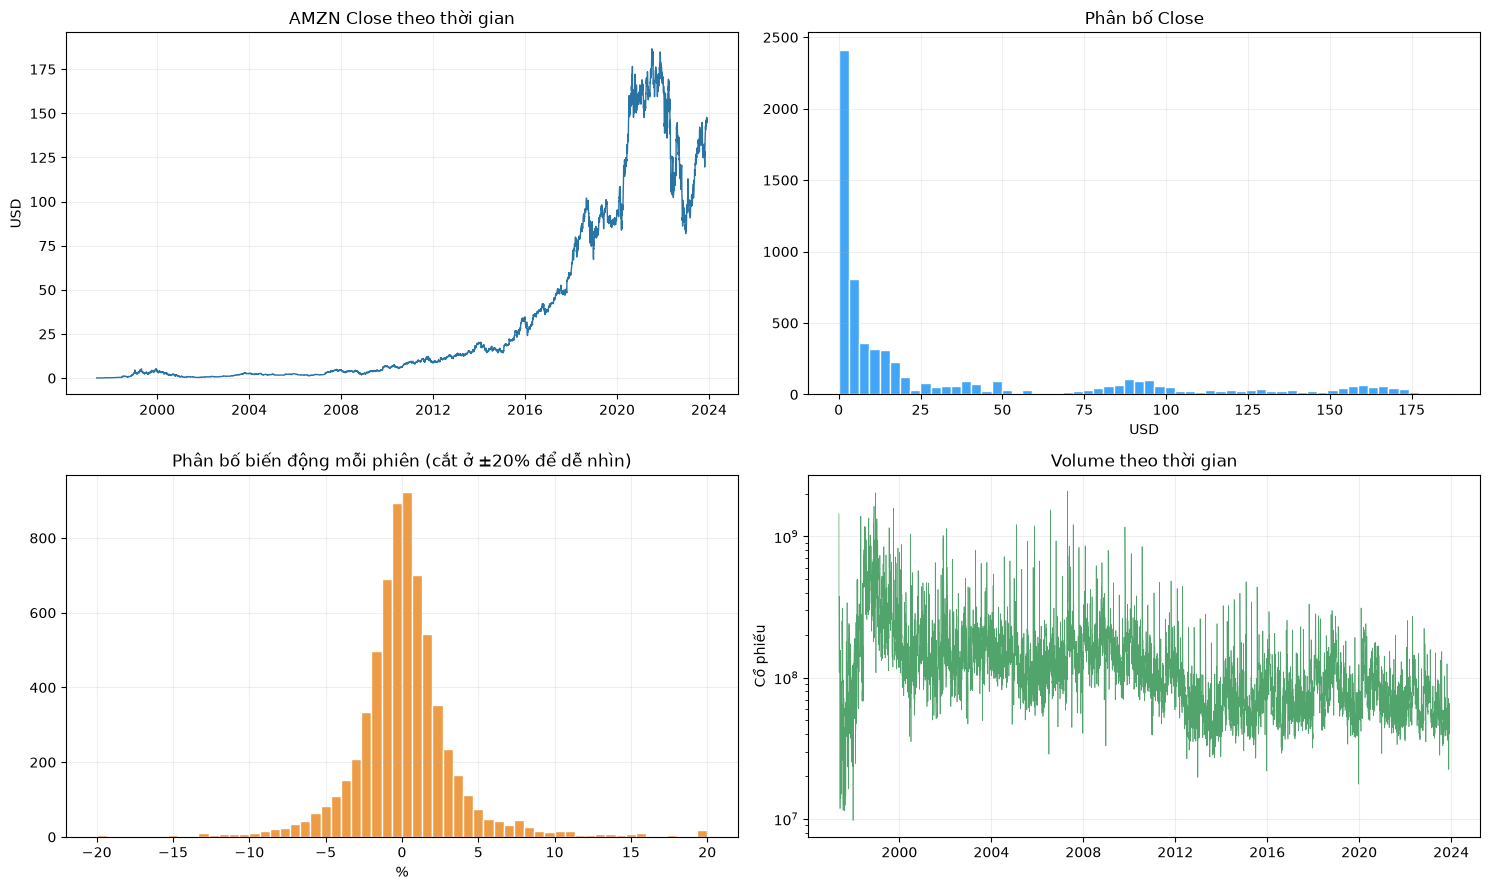
\includegraphics[width=0.93\textwidth]{../Assignment 07/images/generated/amazon_eda_overview.png}
\caption{Khảo sát chuỗi giá, phân bố Close, biến động và Volume của Amazon.}
\label{fig:essay03-a07-amazon-eda}
\end{figure}

Graph có 7.032 node và 7.031 cạnh. Node phiên 05/12/2023 lưu Close
$146{,}880005$ USD, được hiển thị làm tròn thành 146,88 USD. Corpus RAG có 7.005 tài liệu,
ma trận TF-IDF kích thước $7.005\times58.345$. Trong ví dụ truy xuất theo tháng, tài liệu
\texttt{AMZN:month:2023-12} được xếp đầu với điểm cosine $0{,}2643$. Điểm này nói về độ
giống văn bản, không phải độ tin cậy của giá.

\begin{table}[htbp]\centering\color{red}\captionsetup{font={small,essaythreered}}
\caption{Câu hỏi minh họa trên Amazon Stock Price}\label{tab:essay03-a07-amazon}
\begin{tabularx}{\textwidth}{>{\raggedright\arraybackslash}p{4.6cm}>{\raggedright\arraybackslash}Xl}
\toprule
\textbf{Câu hỏi} & \textbf{Trả lời từ dữ liệu} & \textbf{Nhánh}\\
\midrule
Close ngày 05/12/2023? & 146,8800 USD; nguồn \texttt{AMZN:2023-12-05} & Graph\\
Close từ 01 đến 05/12/2023? & 3 phiên; trung bình 146,2500 USD; min 144,8400; max 147,0300 & CSV\\
Tóm tắt dữ liệu Amazon? & 6.684 phiên; nguồn \texttt{AMZN:overview} & RAG + LLM\\
\bottomrule
\end{tabularx}
\end{table}

Giao diện web minh họa hai lối trả lời khác nhau. Hình~\ref{fig:essay03-a07-amazon-kb}
đọc giá của ngày chỉ định từ graph; Hình~\ref{fig:essay03-a07-amazon-rag} dùng tài liệu
tổng quan và Qwen3. Cả hai hiển thị nguồn và công cụ bên dưới câu trả lời.
\begin{figure}[H]\centering\captionsetup{font={small,essaythreered}}
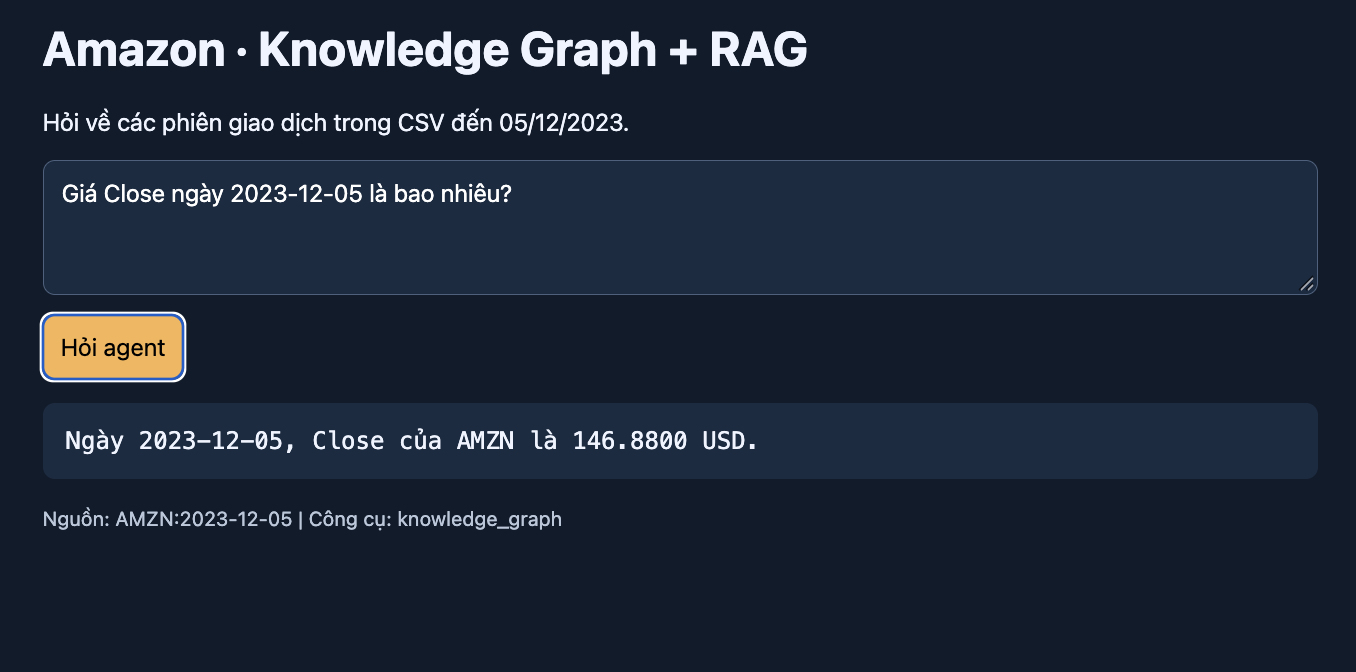
\includegraphics[width=0.88\textwidth]{../Assignment 07/images/deploy/amazon_kb.png}
\caption{Amazon: hỏi Close ngày 05/12/2023 qua Knowledge Graph.}
\label{fig:essay03-a07-amazon-kb}
\end{figure}
\begin{figure}[H]\centering\captionsetup{font={small,essaythreered}}
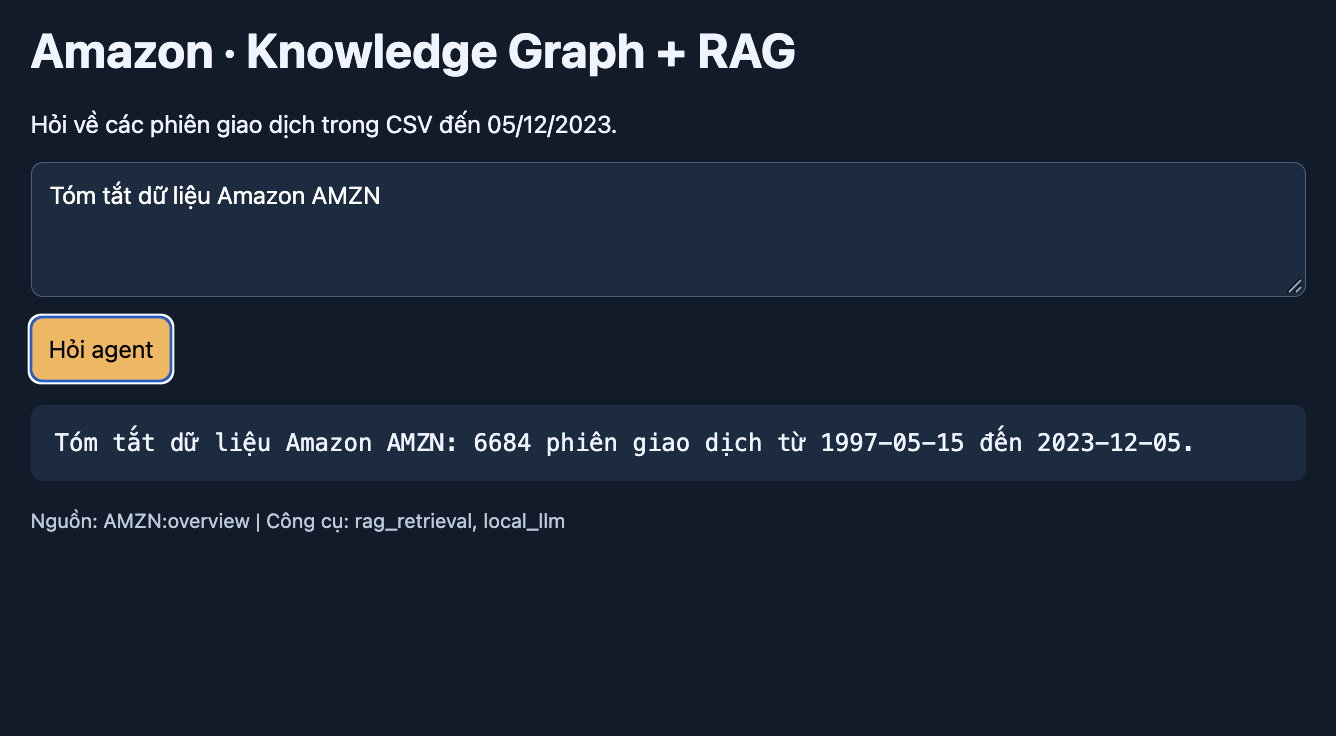
\includegraphics[width=0.88\textwidth]{../Assignment 07/images/deploy/amazon_rag.png}
\caption{Amazon: câu hỏi tóm tắt đi qua RAG và Qwen3.}
\label{fig:essay03-a07-amazon-rag}
\end{figure}

\section{diabetes\_large: hỏi đáp thống kê theo nhóm}
\noindent\textbf{Mã nguồn GitHub: }\url{https://github.com/KhoiF/PTHTTM/tree/main/src/Assignment%2007/diabetes_large}\par
CSV gốc có 100.000 bản ghi với chín cột; \texttt{age\_group} là cột được tạo thêm khi xử lý,
không phải cột thứ mười của CSV. Notebook thấy 3.854 dòng trùng toàn bộ thuộc tính và 8.500
bản ghi nhãn 1, bằng 8,50\%. Các đồ thị EDA mô tả nhãn, tuổi, BMI, HbA1c, glucose cùng một
số nhóm danh mục. Dữ liệu quan sát này không thiết lập nguyên nhân gây bệnh.
\begin{figure}[htbp]\centering\captionsetup{font={small,essaythreered}}
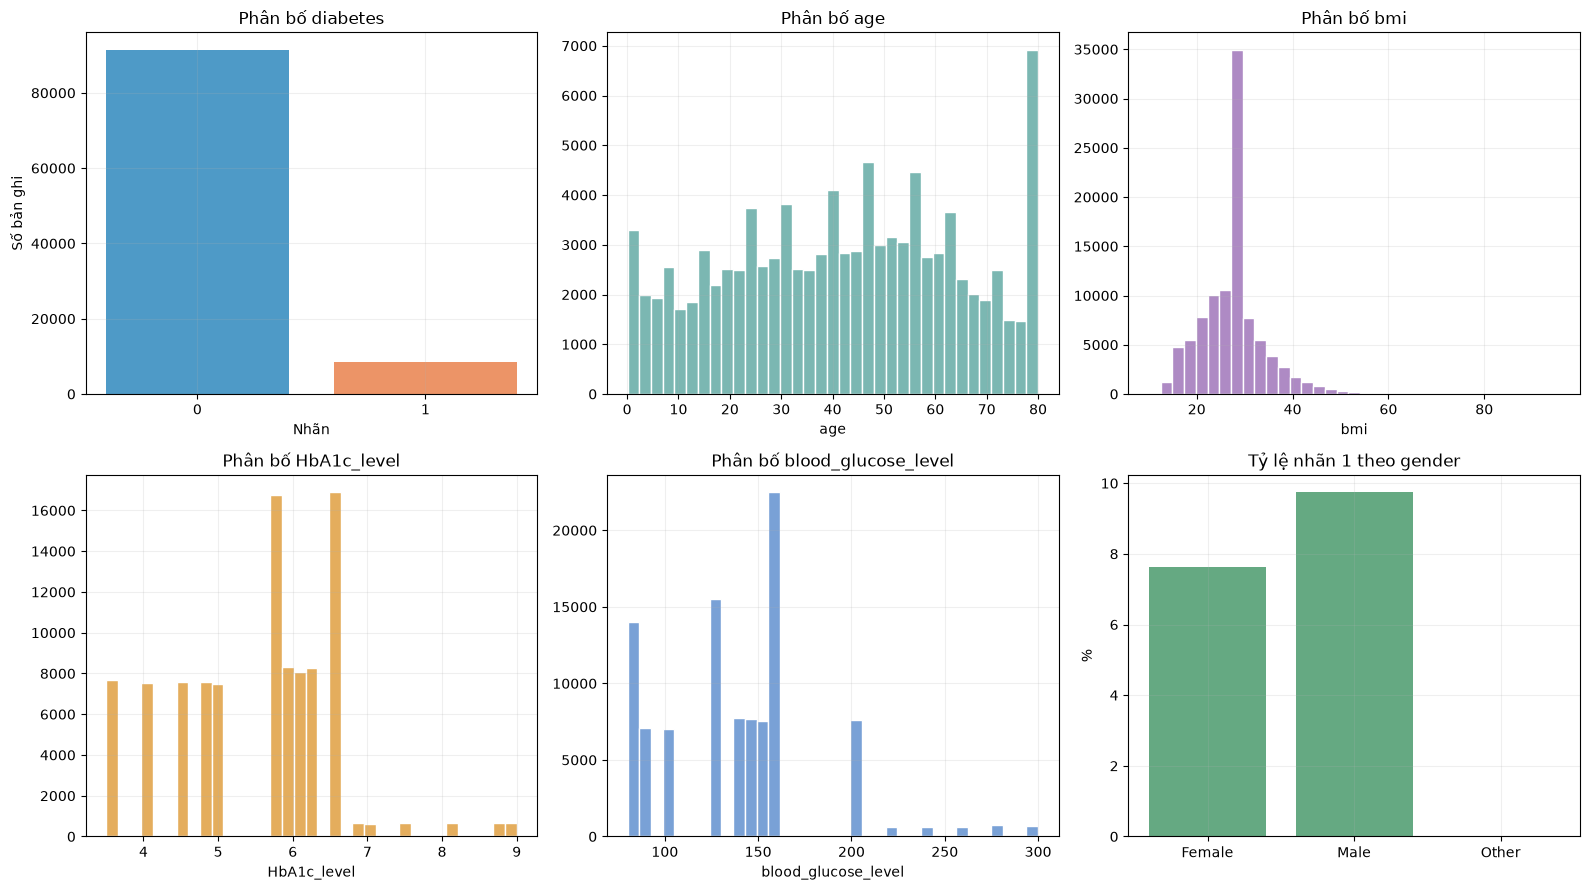
\includegraphics[width=0.93\textwidth]{../Assignment 07/images/generated/diabetes_eda_overview.png}
\caption{Phân bố nhãn và các đặc trưng trong diabetes\_large.}
\label{fig:essay03-a07-diabetes-eda}
\end{figure}

Graph thống kê có 20 node và 51 cạnh; corpus gồm 18 tài liệu, ma trận TF-IDF kích thước
$18\times1.351$. Nhóm nữ có 58.552 bản ghi, 4.461 nhãn \texttt{diabetes=1}, tỷ lệ
7,62\%. Tài liệu \texttt{DIABETES:gender:Female} đứng đầu trong ví dụ truy xuất nhóm nữ
với điểm $0{,}4447$. Tỷ lệ này là số liệu của tập được cung cấp, không phải kết quả
chẩn đoán cho người dùng.

\begin{table}[htbp]\centering\color{red}\captionsetup{font={small,essaythreered}}
\caption{Câu hỏi minh họa trên diabetes\_large}\label{tab:essay03-a07-diabetes}
\begin{tabularx}{\textwidth}{>{\raggedright\arraybackslash}p{4.6cm}>{\raggedright\arraybackslash}Xl}
\toprule
\textbf{Câu hỏi} & \textbf{Trả lời từ dữ liệu} & \textbf{Nhánh}\\
\midrule
Tỷ lệ diabetes ở nữ? & 58.552 bản ghi; 4.461 nhãn 1; 7,62\% & Graph\\
Tỷ lệ toàn dataset? & 100.000 bản ghi; 8.500 nhãn 1; 8,50\% & CSV\\
Tỷ lệ nhóm 60+? & 25.055 bản ghi; 4.932 nhãn 1; 19,68\% & Graph\\
Tóm tắt dataset? & 100.000 bản ghi; nguồn \texttt{DIABETES:overall} & RAG + LLM\\
\bottomrule
\end{tabularx}
\end{table}

Hình~\ref{fig:essay03-a07-diabetes-kb} minh họa câu hỏi theo nhóm được graph xử lý; 
Hình~\ref{fig:essay03-a07-diabetes-rag} minh họa câu hỏi tóm tắt từ tài liệu tổng quan.
Giao diện nhắc rõ rằng thống kê không dùng để chẩn đoán.
\begin{figure}[H]\centering\captionsetup{font={small,essaythreered}}
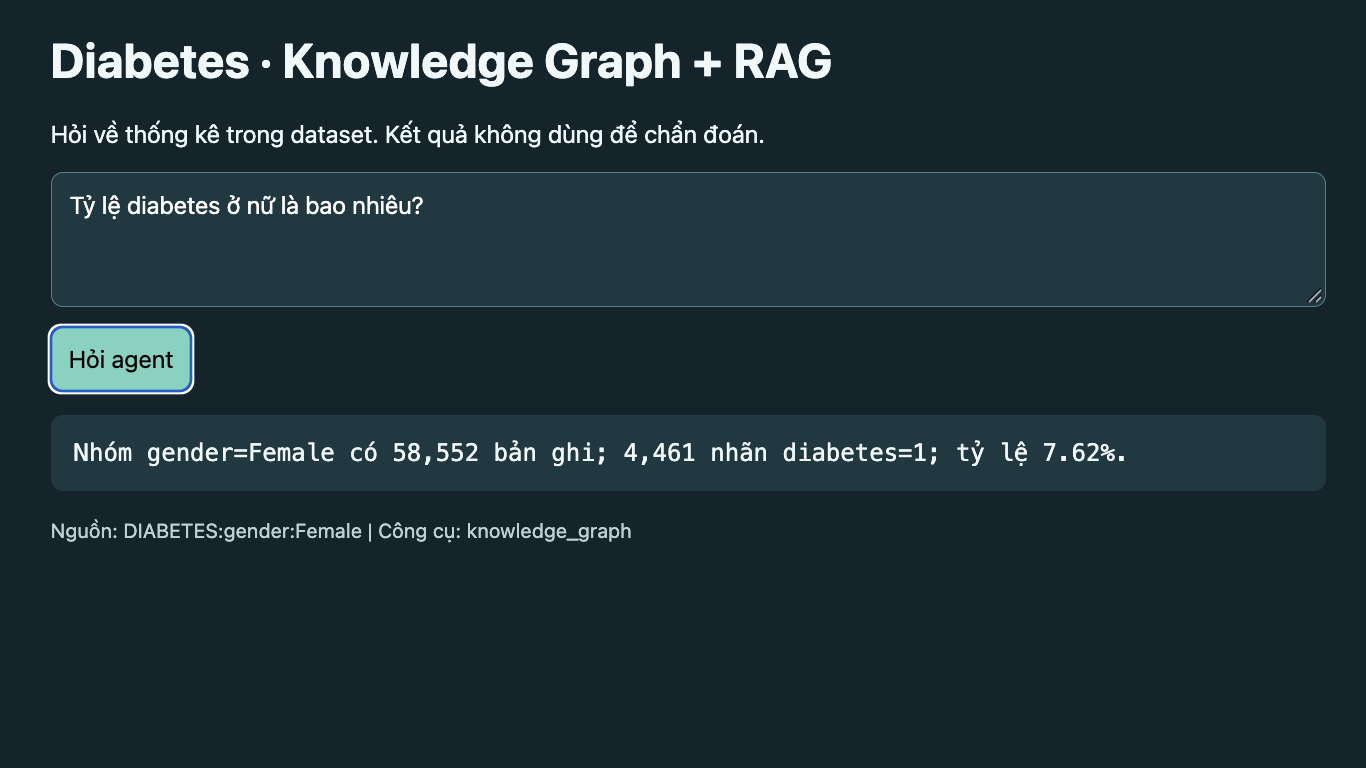
\includegraphics[width=0.88\textwidth]{../Assignment 07/images/deploy/diabetes_kb.png}
\caption{Diabetes: tỷ lệ nhãn 1 ở nữ được trả từ Knowledge Graph.}
\label{fig:essay03-a07-diabetes-kb}
\end{figure}
\begin{figure}[H]\centering\captionsetup{font={small,essaythreered}}
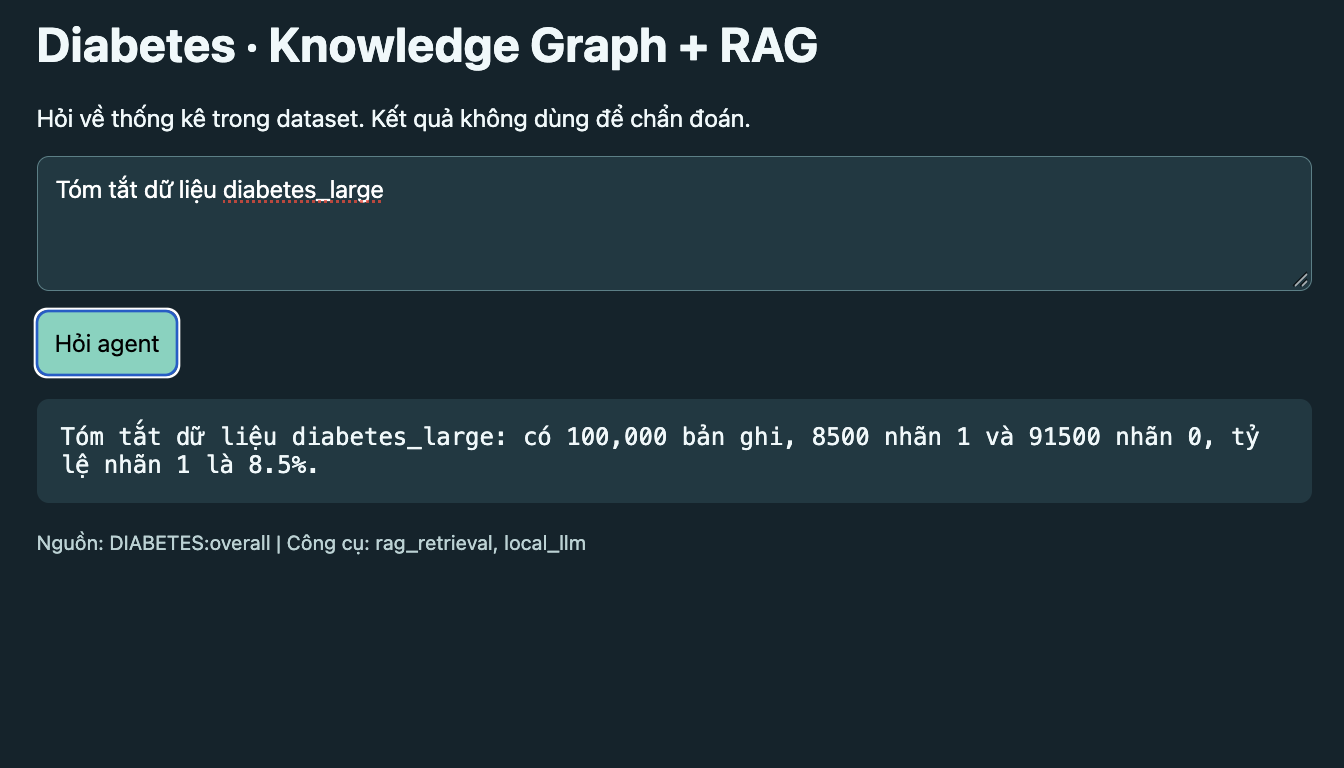
\includegraphics[width=0.88\textwidth]{../Assignment 07/images/deploy/diabetes_rag.png}
\caption{Diabetes: câu hỏi tóm tắt đi qua RAG và Qwen3.}
\label{fig:essay03-a07-diabetes-rag}
\end{figure}

\section{Triển khai và giới hạn}
Hai ứng dụng có lệnh CLI \texttt{--question} và giao diện Flask \texttt{--web} trên localhost;
Amazon dùng cổng mặc định 8007, diabetes dùng 8008. API nhận câu hỏi và trả câu trả lời, nguồn
cùng công cụ đã dùng. Graph và phép tính CSV không cần nạp Qwen3; nhánh RAG mới nạp mô hình khi
cần. Việc đưa LLM vào câu hỏi mô tả không biến hệ thành công cụ dự báo giá hay phân loại bệnh
của các Assignment trước.

TF-IDF ký tự phụ thuộc mức giống bề mặt giữa câu hỏi và tài liệu. Nếu cách diễn đạt khác xa
corpus, tài liệu đúng có thể không được tìm thấy; nếu truy xuất được tài liệu gần từ vựng,
mô hình vẫn có thể lược bỏ chi tiết. ID nguồn giúp kiểm tra lại nhưng không tự bảo đảm
groundedness. Giá Amazon kết thúc ở 05/12/2023; tỷ lệ diabetes chỉ mô tả dữ liệu quan sát.
Ứng dụng do đó thích hợp để minh họa hỏi đáp và thống kê trên hai CSV, không dùng cho quyết định
đầu tư hoặc chẩn đoán y khoa.

\clearpage
\endgroup
\hypersetup{linkcolor=blue!70!black,urlcolor=blue!70!black,citecolor=blue!70!black}

\clearpage
\begin{thebibliography}{99}
\addcontentsline{toc}{chapter}{Tài liệu tham khảo}
\bibitem{turing1950} A. M. Turing, ``Computing Machinery and Intelligence,'' \textit{Mind}, 1950. \url{https://academic.oup.com/mind/article/LIX/236/433/986238}.
\bibitem{dartmouth1955} J. McCarthy, M. Minsky, N. Rochester và C. Shannon, ``A Proposal for the Dartmouth Summer Research Project on Artificial Intelligence,'' 1955. \url{https://www-formal.stanford.edu/jmc/history/dartmouth/dartmouth.html}.
\bibitem{rosenblatt1958} F. Rosenblatt, ``The Perceptron: A Probabilistic Model for Information Storage and Organization in the Brain,'' \textit{Psychological Review}, 1958. \url{https://doi.org/10.1037/h0042519}.
\bibitem{rumelhart1986} D. Rumelhart, G. Hinton và R. Williams, ``Learning representations by back-propagating errors,'' \textit{Nature}, 1986. \url{https://doi.org/10.1038/323533a0}.
\bibitem{alexnet2012} A. Krizhevsky, I. Sutskever và G. Hinton, ``ImageNet Classification with Deep Convolutional Neural Networks,'' \textit{NeurIPS}, 2012. \url{https://proceedings.neurips.cc/paper/2012/hash/c399862d3b9d6b76c8436e924a68c-Abstract.html}.
\bibitem{transformer2017} A. Vaswani và cộng sự, ``Attention Is All You Need,'' \textit{NeurIPS}, 2017. \url{https://arxiv.org/abs/1706.03762}.
\bibitem{resnet2016} K. He và cộng sự, ``Deep Residual Learning for Image Recognition,'' \textit{CVPR}, 2016. \url{https://openaccess.thecvf.com/content_cvpr_2016/html/He_Deep_Residual_Learning_CVPR_2016_paper.html}.
\bibitem{bengio1994} Y. Bengio, P. Simard và P. Frasconi, ``Learning Long-Term Dependencies with Gradient Descent is Difficult,'' \textit{IEEE Transactions on Neural Networks}, 1994. \url{https://doi.org/10.1109/72.279181}.
\bibitem{cifar10} A. Krizhevsky, V. Nair và G. Hinton, ``CIFAR-10 and CIFAR-100 datasets.'' \url{https://www.cs.toronto.edu/~kriz/cifar.html}.
\bibitem{project} P. V. Khôi, mã nguồn và báo cáo Assignment 03, 04, 06, 07 của project \textit{PTHTTM}. \url{https://github.com/KhoiF/PTHTTM}.

\bibitem{essay03-w3c} W3C, \textit{RDF 1.1 Concepts and Abstract Syntax}, 2014.
\url{https://www.w3.org/TR/rdf-concepts/}.
\bibitem{essay03-google} A. Singhal, Google, \textit{Introducing the Knowledge Graph: things, not strings}, 2012.
\url{https://blog.google/products-and-platforms/products/search/introducing-knowledge-graph-things-not/}.
\bibitem{essay03-lewis} P. Lewis và cộng sự, \textit{Retrieval-Augmented Generation for Knowledge-Intensive NLP Tasks}, 2020.
\url{https://arxiv.org/abs/2005.11401}.
\bibitem{essay03-qwen} Qwen, \textit{Qwen3-0.6B Model Card}.
\url{https://huggingface.co/Qwen/Qwen3-0.6B}.
\bibitem{essay03-graphrag} D. Edge và cộng sự, \textit{From Local to Global: A Graph RAG Approach to Query-Focused Summarization}, 2024.
\url{https://arxiv.org/abs/2404.16130}.
\end{thebibliography}
\end{document}
